\documentclass[12pt, notitlepage]{report}
\usepackage[utf8]{inputenc}
\usepackage[margin = 1in]{geometry}
\usepackage{amsmath}
\usepackage{rotating}
\usepackage{biblatex}

\usepackage{setspace}
\onehalfspacing

\addbibresource{references.bib}


\title{
{Thesis Proposal:}\\
{Three Studies on the Brittle Response to Earthquake Stressing} \\
{\large University of California Santa Cruz}
}
\date{March 2019}
\author{Kelian Dascher-Cousineau}

\begin{document}


\maketitle

\tableofcontents{}

\chapter*{Preface}

Enclosed the readers will find a three-part research proposal to be completed over three years. I intend to acquire a robust foundation in earthquake physics and fault mechanics while covering a diversity of topics including earthquake statistics, geomorphology, and machine learning. Chapter \ref{cpt:productivity} outlines an analysis of global patterns in the number of aftershocks produced by an earthquake. The work presented in this chapter is nearing completion. Chapter \ref{cpt:damage} outlines some preliminary results in remotely detecting fault damage. To do so, I couple landscape metrics derived from high-resolution lidar with landscape evolution models. Chapter \ref{cpt:ML} is a work plan to use a deep learning approach to assess short term earthquake rate instead of traditional statistical models. Finally, chapter \ref{cpt:plan} provides a timeline to completion with significant anticipated milestones. The proposed thesis project explores the brittle response of the earthquake crust to earthquake stressing. Throughout, I relate physical insights to tangible improvements in earthquake-hazard assessment. 
\\
\\
Enjoy!
\\
Kelian Dascher-Cousineau

\newpage
 
\chapter{Global patterns in aftershock productivity}\label{cpt:productivity}

\begin{abstract}
The number of aftershocks generated by an earthquake is generally related to the size of the mainshock. However, aftershock sequences can have significant excursions from a simple magnitude-dependent productivity law. This variability is particularly concerning for great earthquakes where the number of damaging aftershocks can vary by factors of 40 for mainshocks of comparable magnitude. We capitalize on the recent finding that strike-slip earthquakes produce fewer aftershocks at a given magnitude than dip-slip earthquakes to determine mainshock characteristics that govern productivity variations. Is the paucity of aftershocks for strike-slip earthquakes a location effect or an effect of the rupture itself? We decluster the global catalog and count aftershock using space-time windowing to measure productivity. We examine its variations in the context of its tectonic setting, rupture properties, and source geometry. We show that faulting type exhibits little variation when we control for location. We find that the age of the lithosphere correlates well with earthquake productivity. We proceed to build a catalog of earthquake source parameters based on the finite fault source inversions by Hayes et al. [2017] for the great-sized earthquakes from 1990 to 2017. We tabulate source dimensions, seismic energy, and new measurements of heterogeneity and stress drop. The compilation highlights that particularly long and narrow ruptures, have markedly lower productivity. Building upon recent findings, we interpret high stress drops to indicate slip over a smaller area, smaller activated volumes, and, therefore, fewer aftershocks. Our results reinforce that the availability of faults and source geometry are first-order features of aftershock triggering.
\end{abstract}


\section{Introduction}
Earthquakes cluster in time and space \cite{Omori1895}. In a sequence, the largest earthquake is the mainshock, those preceding are foreshocks, and those following are aftershocks. Earthquake clustering indicates how the lithosphere transmits stresses on timescales of seconds to years \cite{felzer2006decay, Stein1999, Scholz2019TheFaulting, Shebalin2017}. The Gutenberg-Richter law, Omori's law, and the productivity law statistically describe coarse features of the evolution of earthquake sequences, respectively capturing the magnitude-frequency scaling, the temporal decay, mainshock magnitude dependence of an earthquake sequence  \cite{deArcangelis2016StatisticalForecasting, Helmstetter2003BathsProperties, GutenbergBulletinAmerica,Omori1895}. Epidemic-Type Aftershock Sequence (ETAS) \cite{Kagan1981StochasticCatalogs,Ogata1988} and similar statistical models \cite{Holliday2008ABASS}, combine the statistical empiricism in holistic statistical frameworks \cite{ogata2017statistics}. All earthquakes have aftershocks and contribute to increasing the underlying rate of earthquakes. The probability of an earthquake aftershock exceeding the magnitude of an original mainshock, the size of the largest aftershock, along with the spatial reach of an earthquake sequence all map from these basic statistical features \cite{Helmstetter2003BathsProperties, Reasenberg1999ForeshockEarthquakes}.

The phenomenology of earthquake aftershocks under-constrains the underlying physical process transferring the earthquakes stress through the crust. Underlying physical models are non-unique and difficult to discriminate. Stress corrosion \cite{Das1981}, fluid migration \cite{Nur1972AftershocksFlow,Ross2017AftershocksMesh}, Coulomb stress change \cite{Stein1999} and dynamic triggering \cite{felzer2006decay} all reproduce empirical laws governing aftershocks sequences \cite{Scholz2019TheFaulting}. More observations are necessary.

We focus on a component of this statistical framework. \textit{Earthquake productivity} is a measure of the tendency of an earthquake to generate aftershocks. The number of aftershocks in any given sequence scales with the magnitude of the mainshock:
\begin{equation}\label{eq:productivity}
    log\hat{N} = log(k)+\alpha(M-M_o)
\end{equation}
where $\hat{N}$ is the expected number of aftershocks, $k$ is a constant, $\alpha$ is a scaling exponent typically near unity, $M$ is the magnitude and $M_o$ is the magnitude of completeness \cite{deArcangelis2016StatisticalForecasting}. In bulk, the scaling relationship is remarkably robust \cite{deArcangelis2016StatisticalForecasting, Kisslinger2011AftershocksProperties,Tahir2015,Tahir2014Aftershock2005,Page}. However, individual earthquake sequences exhibit significant, order of magnitude, excursions from the scaling relationship.% A basic physical interpretation of variability in the number of aftershocks involves a mainshock's ability to trigger (or suppress) earthquakes and the susceptibility of the surrounding lithosphere \cite{Mogi1967EarthquakesFractures,Stein1999,Dieterich1994}. Larger earthquakes trigger more aftershocks, however, significant excursions from a simple magnitude-scaling law exist implying that different groups of earthquakes are subject to different statistical laws and underlying physics. 
Regional patterns indicate that this variability is not just a result of the stochasticity of the crustal system. For example the productivity of Eastern and Western Pacific \cite{Singh1988Regionalle7.0, Wetzler2016} are distinct. The confluence of such observations has led some to segment earthquake statistics to a regional basis \cite{ChuComparisonZones, Page, Davidsen2015GeneralizedCalifornia, Tahir2014Aftershock2005, ogata2017statistics}. These approaches have significantly advanced hazard assessment \cite{Page, deArcangelis2016StatisticalForecasting, ogata2017statistics}. However, this general approach does not address the core reasons that cause variability in aftershock productivity. To this avail, we will find physical motivations to segment the catalog. 

The number of aftershocks and, by extension, the size of the largest earthquake tends to be smaller for strike-slip earthquakes \cite{Tahir2012,Tahir2014Aftershock2005,Tahir2015}. This observation is a starting point to probe the underlying physics of aftershock phenomenology. 

Strike-slip earthquakes tend to have longer rupture duration \cite{Houston2001InfluenceFunctions}, have longer aspect ratios \cite{Hayes2017}, are well known to occur on transform faults, have higher stress drop \cite{Allmann2009GlobalEarthquakes}, can host supershear ruptures \cite{Bouchon2008TheEarthquakes}, have lower background seismicity \cite{Tahir2015}, have higher b-values and follow distinct scaling relationships \cite{Scholz2019TheFaulting}. These physical distinctions yield observationally motivated, physically justified and testable hypotheses to identify controls on the aftershock productivity of earthquakes.

We explore why faulting style appears to affect the number of aftershocks using global catalogs along with finite fault inversions of major earthquakes since 1990. We extend the analysis to a lower magnitude of completeness and provide an overview of global patterns of productivity that arise from our analysis. We test two overarching hypotheses --- strike-slip earthquake are deficient in aftershocks because of 1) a type regional setting or 2) characteristic source parameters. We find evidence indicating that productivity is not inherent to the faulting style; instead, the geometry of the source and the availability of stressed faults determine first-order variations on earthquake productivity.


\section{Methods}
\subsection{Relative productivity}

To characterize the relative productivity of earthquakes, we build off of the productivity law (Equation \ref{eq:productivity}). An earthquake is more or less productive based on its \textit{relative productivity}, $N^*$:

\begin{equation}{\label{eq:residual_productivity}}
    N^*_i = logN_i - log(\hat{N}) = log\left(\dfrac{N}{k10^{\alpha(M-M_o)}}\right)
\end{equation}
We will use the relative productivity of earthquakes extensively to compare and contrast different subsets of the global catalog. 
An accurate estimate of $N^*$ requires many aftershocks. An exponential representation of aftershock productivity is poorly resolved for earthquakes with few detected aftershocks ($<10$). An earthquake with no aftershocks cannot be described by equation \ref{eq:residual_productivity} where $N^*(N=0) = -\infty$.

We leverage the Incorporated Research Institutions for Seismology (IRIS) data management services to aggregate catalogs of global seismicity and focal mechanism solutions. We combine all earthquakes available in the National Earthquake Information Center catalog (NEIC) and the International Seismological Center (ISC). We only use moment magnitude estimates ($M_w$). These catalogs supply an additional order of magnitude of earthquakes to study. Conservative estimates from \textcite{Woessner2005AssessingUncertainty}  find that the global catalog from 1980 to 2000 is complete to a range of $4.3 < M_w < 5$. We choose a completeness of $M_w4.5$ for all earthquakes from 1980 to 2019. 

Sensitivity tests of significant results to the magnitude of completeness guard against regional patterns in catalog completeness, should they arise. Where available, focal mechanism solutions from the NEIC and Harvard Global Centroid Moment Tensor (gCMT) catalogs, with preference to the former, are joined to the global earthquake catalog. We categorize focal mechanisms (strike-slip, normal, and reverse) using the pressure (P) and tension (T)axes supplied in the inversion of the NEIC and gCMT catalogs. IRIS data management service ID's are used to attribute focal mechanisms to their respective earthquakes correctly. 

\subsection{Space-time windowing}

Schemes with varying levels of sophistication identify earthquakes foreshocks, mainshocks, and aftershocks — analyses trade-off robustness and transparency. We follow a simple space-time windowing scheme--- here we prefer transparency as it allows for easier troubleshooting and interpretation of results. The choice will have little influence on the qualitative conclusions of similar analyses \cite{Utsu1995}.

Stepping down in magnitude from the largest earthquake in the catalog to catalog completeness, we classify earthquakes as aftershocks if they are within three sources dimensions from the mainshock and 60 days from the mainshock. To prevent misattributing aftershocks to other earthquake sequences, we flag earthquakes within four source dimensions and 100 days after the mainshock. Potential foreshocks within four source dimensions and a day before the mainshock are also flagged. Source dimension estimates follow \textcite{Wells1994}: $R\sim10^{0.59M}$. For reference, $M_w$ 6 and nine earthquakes have dimensions on the order of $\sim 20$ km and $\sim 500$ km respectively. Aftershocks and flagged earthquakes are removed from the catalog to avoid double counting earthquakes in subsequent sequences. The result is a declustered catalog recording the number of aftershocks of each mainshock. 

We use the median number of aftershocks for each 0.1 magnitude bin in the declustered catalog and the corresponding magnitude to perform a linear least squares inversion to determine the $ log k - \alpha M_o $ and $\alpha$ given the median number of aftershocks. Using these parameters, we determine the relative productivity ($N^*$) for all earthquakes in our catalog from equation  \ref{eq:residual_productivity}.

\begin{sidewaysfigure}[!p]
    \centering
    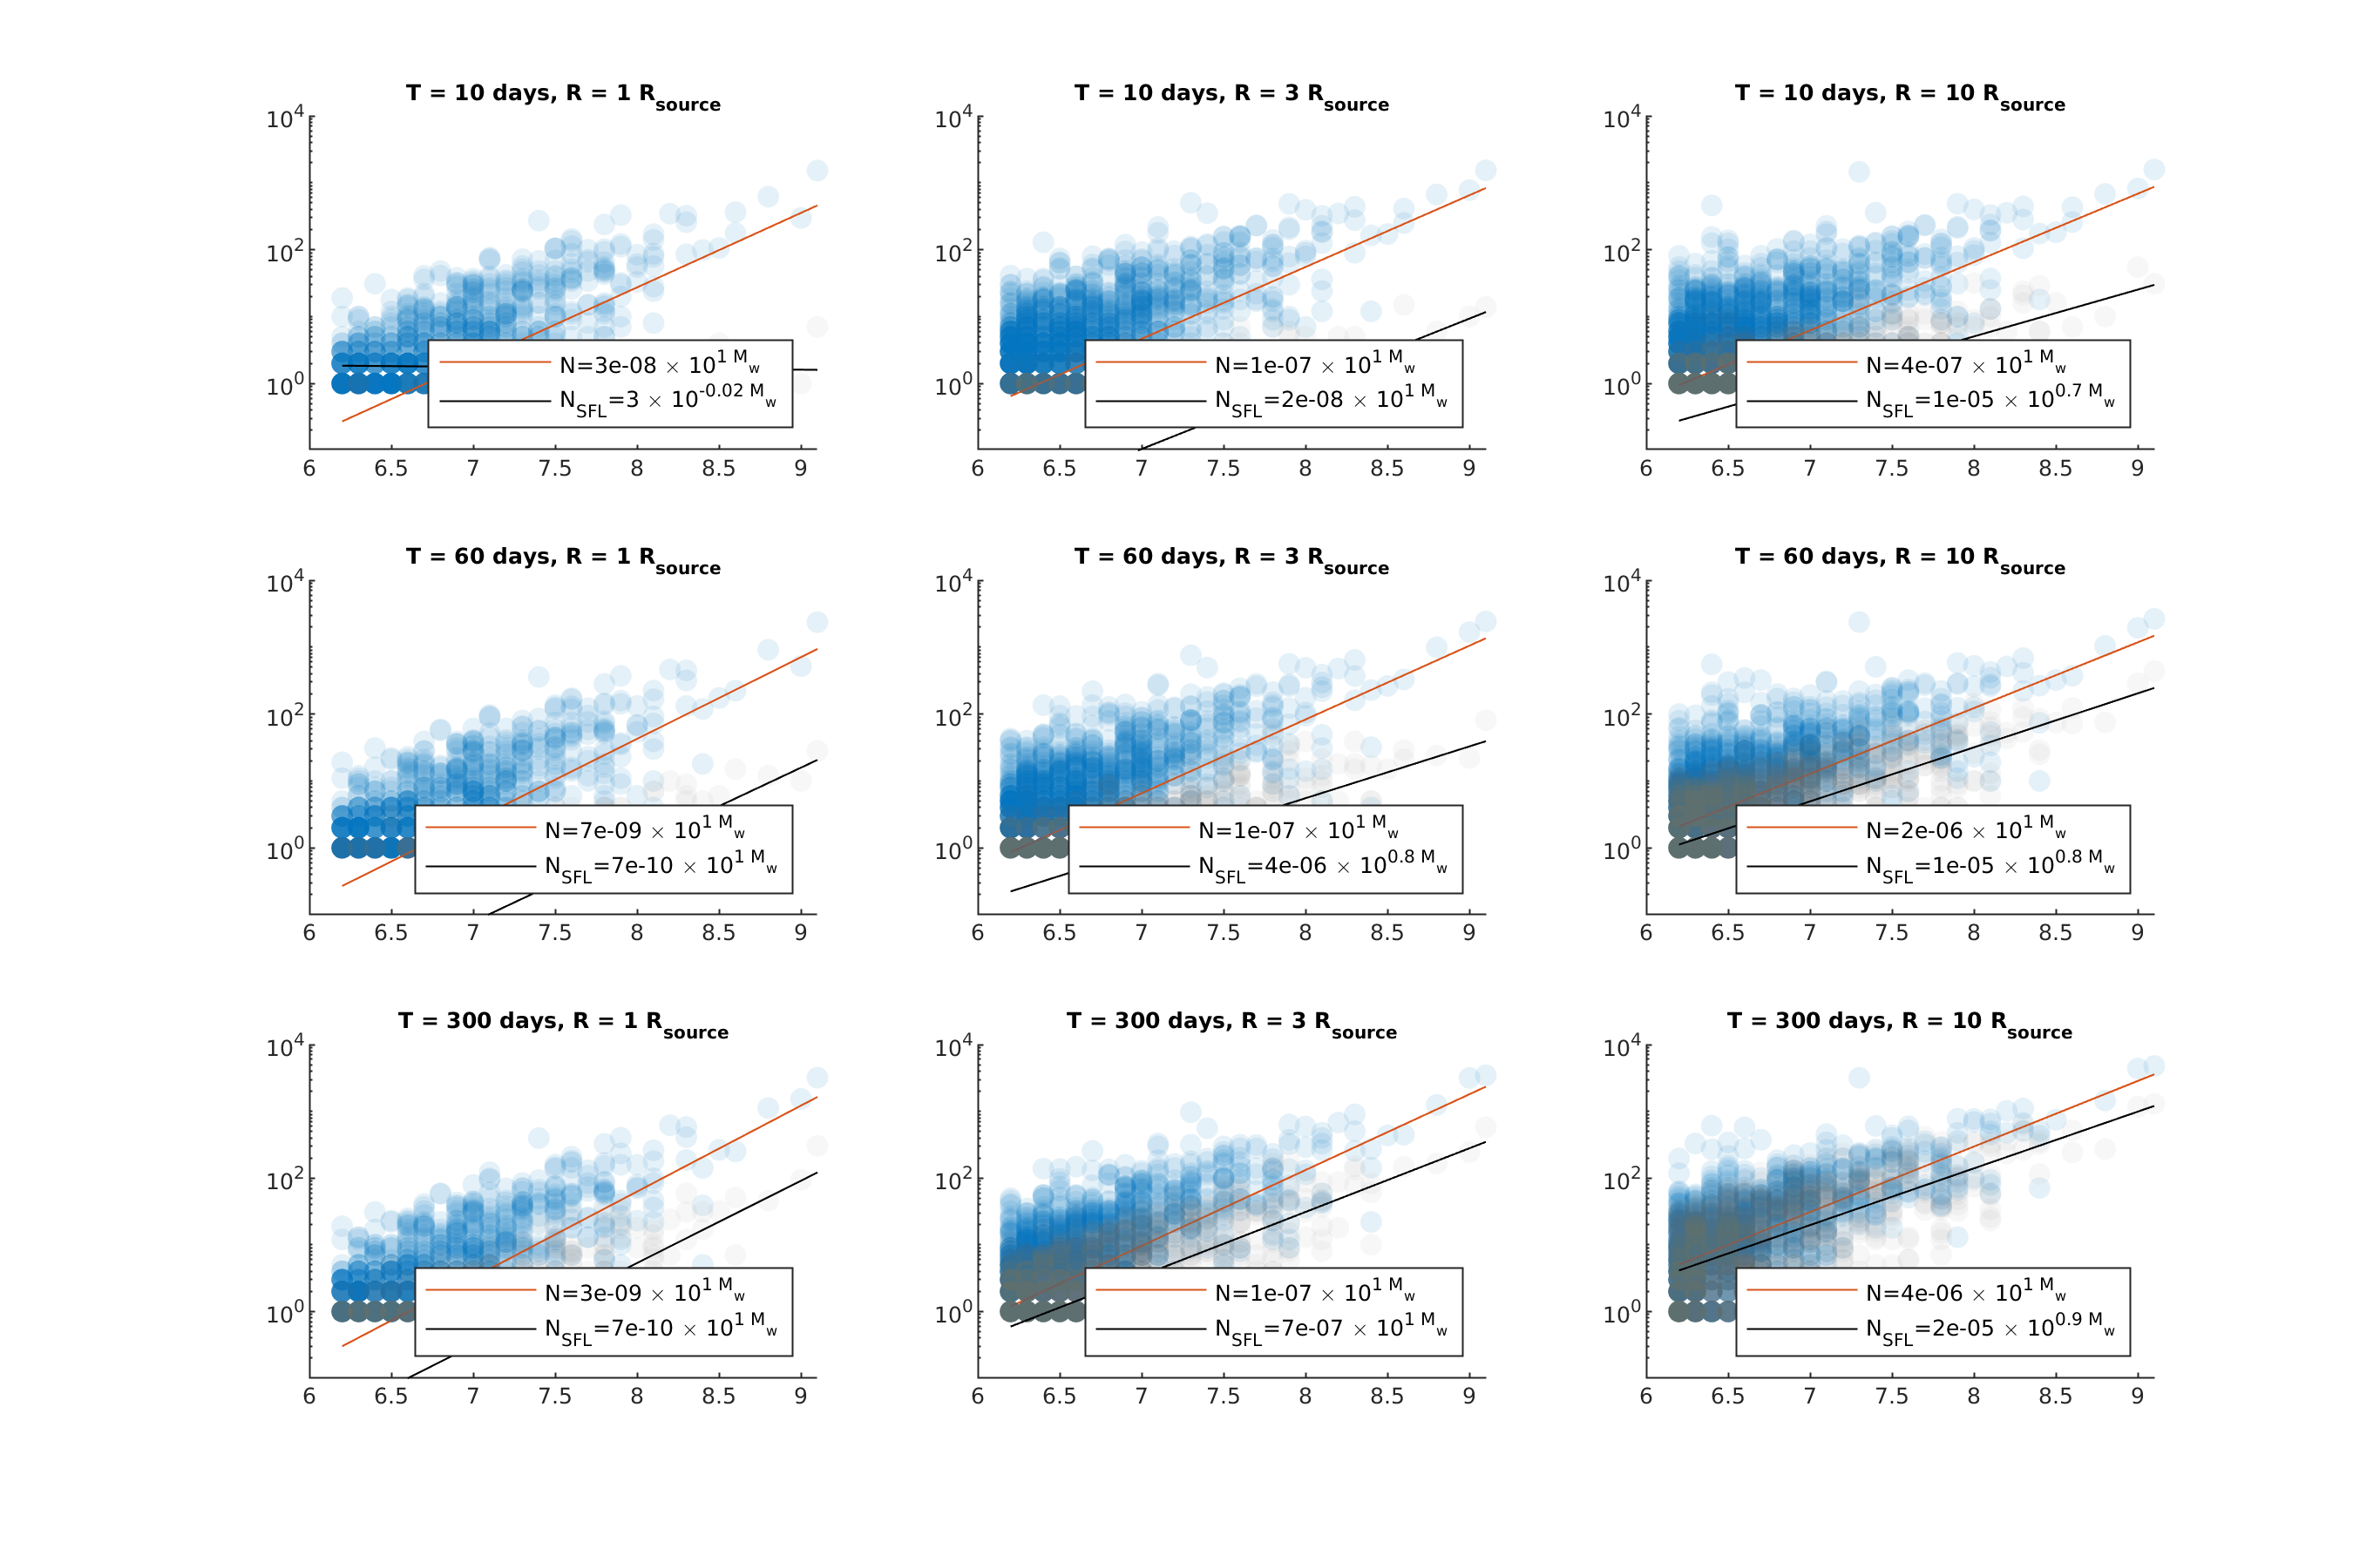
\includegraphics{figures/space_time_sensitivity.png}
    \caption{Sensitivity analysis for the choice of space-time windows. Blue data are mainshocks identified through our hierarchical declustering routine. Regressions are computed using least squares through the log-transformed median values for each magnitude bin. Grey points show mainshock identified following the same approach, but for a shuffled catalog, that is a catalog a shuffled time vector. Note that as space and time windows are made larger, the likelihood of simply measuring background productivity in the productivity law becomes an increasing concern.}
    \label{fig:sensitivity}
\end{sidewaysfigure} 

The choice of time and space window is rather subjective. Smaller windows increase the certainty that aftershocks are correctly attributed. Larger time windows include more aftershocks yielding more stable estimates of the relative productivity of aftershocks sequences. We prefer large windows to ensure that the relative productivity is well estimated. Figure \ref{fig:sensitivity} shows the sensitivity of the number of aftershocks and the magnitude scaling to different space-time window. We also include a shuffle test that validates that the productivity law is not an artifact of the space time windowing. Visual inspection of individual sequences and global $\alpha$-values near unity are an additional affirmation that aftershocks are not misattributed (at least to the extent that results would be affected significantly).

\section{Focal mechanism dependence of aftershock productivity}

Our analysis yields 2662 earthquake sequences, of which we categorize 2372  focal mechanism types. We refine the analysis of \textcite{Tahir2015} showing a clear separation of earthquake productivity by focal mechanism (see Figure \ref{fig:fms_prod}). Strike-slip mainshocks exhibit the least amount of aftershocks with a relative productivity of -0.4 or, equivalently, three times fewer than dip-slip focal mechanisms. This separation by focal mechanism far exceeds 95\% confidence intervals ($p\ll $ 0.05). 

\begin{figure}[!ht]
    \centering
    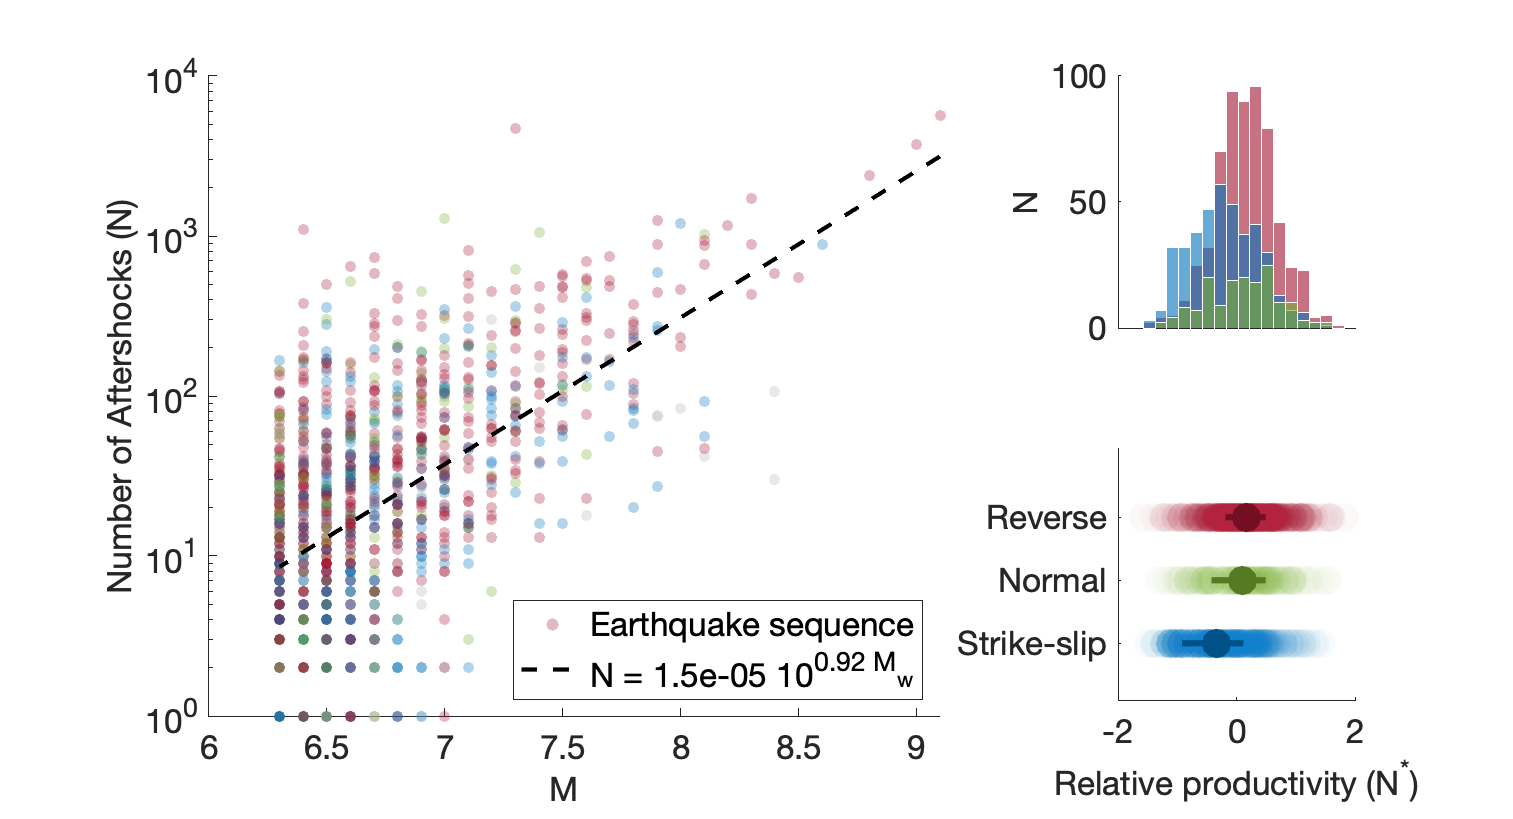
\includegraphics[width = \textwidth]{figures/fms_prod.eps}
    \caption{Left: Earthquake productivity as a function of mainshock magnitude. Focal mechanism type is color-coded such that blue, green and red points correspond to earthquake sequences for which the mainshock was respectively strike-slip, normal and reverse. The dashed line indicates the global productivity law. Note that strike-slip mainshocks tend to have fewer aftershocks for any magnitude than do either dip-slip mechanisms. Right: Panels highlight the distribution of relative productivity as a function of focal mechanism.}
    \label{fig:fms_prod}
\end{figure}

\section{The global earthquake productivity map}

We map the global catalog of aftershock productivity (Figure \ref{fig:global_res}). This section provides an overview of first-order features along with notable regional patterns. These observations provide a footing to motivate the analysis to come.

\textit{Deep earthquakes.} Long continental scale bands of earthquakes with low relative productivity run parallel to the Atacama, Japan, Izu-Ogasawara, Mariana and Tonga trenches (see for example Figure \ref{fig:atacama}). These earthquakes share both normal and reverse dip-slip focal mechanisms. Upon inspection, they are very deep-focus earthquakes ($>100$ km in depth). We do not include these earthquakes in the subsequent analysis to avoid confounding other possible controls with a  a depth signal (see figure \ref{fig:prod_vs_depth}

\begin{figure}
    \centering
    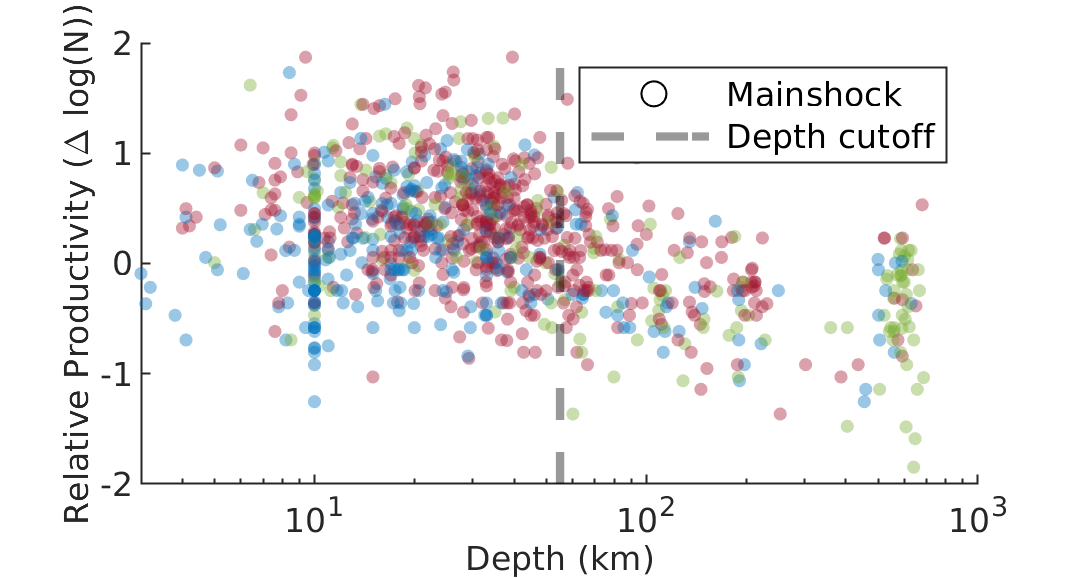
\includegraphics{figures/prod_vs_depth.png}
    \caption{Earthquake relative productivity as a function of depth. Note that there appears to be a marked decrease in earthquake productivity as a function of depth. Subsequent analysis will only consider earthquakes shallower than 55 km in depth. Sequences are color-coded by faulting style of the mainshock (blue: strike-slip, green: normal and red: reverse).}
    \label{fig:prod_vs_depth}
\end{figure}

\textit{Oceanic transform and divergent boundaries.} A quick overview of the global productivity map indicates that earthquake offshore, removed from subduction zones have fewer aftershocks. Mainshocks along oceanic transform and divergent boundaries are nearly systematically less productive than the global trend ($N^*<0$). We find few exceptions; the $M_w8.6$, 2012, strike-slip rupture offshore Sumatra followed by a $M_w8.2$ aftershock appears to be among the most productive earthquakes hosted in oceanic lithosphere, not within a convergent boundary. Neither the mainshock or the aftershocks ruptured along known tectonic boundaries. % Whether strike-slip earthquakes are deficient in aftershocks because they are hosted in oceanic lithosphere or whether the opposite is true is difficult to assess. 

\textit{The North-American Coast.} We note some remarkable spatial coherency in the relative productivity of earthquakes along the North American Coast. The Aleutian arc grades from earthquakes with varying but generally high productivity in the West to low productivity in the East. The recent North-Eastern Pacific Earthquakes which fractured a relic shatter zone appears to have generally higher productivity. Earthquakes on the Queen Charlotte Fault offshore western Canada are coherent and exhibit below-average productivity. Clusters of seismicity associated with the Blanco shatter zone and the Mendocino triple junction has similarly low productivity. Continental earthquakes of the San Andreas are markedly more productive than the seismicity to the North and South. A stark decrease in productivity seems to correspond, to a shift from generally convergent tectonic hosted on land to extensional tectonics to the south along the Baja California Peninsula. Subduction of the northernmost section of the Cocos plate under Mexico is generally associated with lower aftershock productivity, though the rate of aftershocks increases southward in central America. 

Variability along the entire continental boundary appears to coarsely correlate with abrupt changes in tectonic setting and the age of the oceanic lithosphere. Most notable is the pronounced distinction in productivity associated with the San Andreas. Where the lithosphere is young aftershocks are scarce; older lithosphere appears to be associated with the occurrence of more aftershocks.

%\textit{The Sandwich.} 

%\textit{The Marianas Trench.}

%\textit{New Zeland.}

\textit{Continental Seismicity.} We note that continental seismicity tends to be associated with higher relative productivity with a relative productivity almost systematically exceeding the global average. Notably, the seismicity described by \textcite{Tahir2014Aftershock2005} of the India-Asia Collision Belt generally looks to have higher productivity (see Figure \ref{fig:continental}). Other examples of high continental productivity include onshore seismicity in New-Zealand, the San Andreas Fault, and the Arabian Plate collision.

\begin{figure}
    \centering
    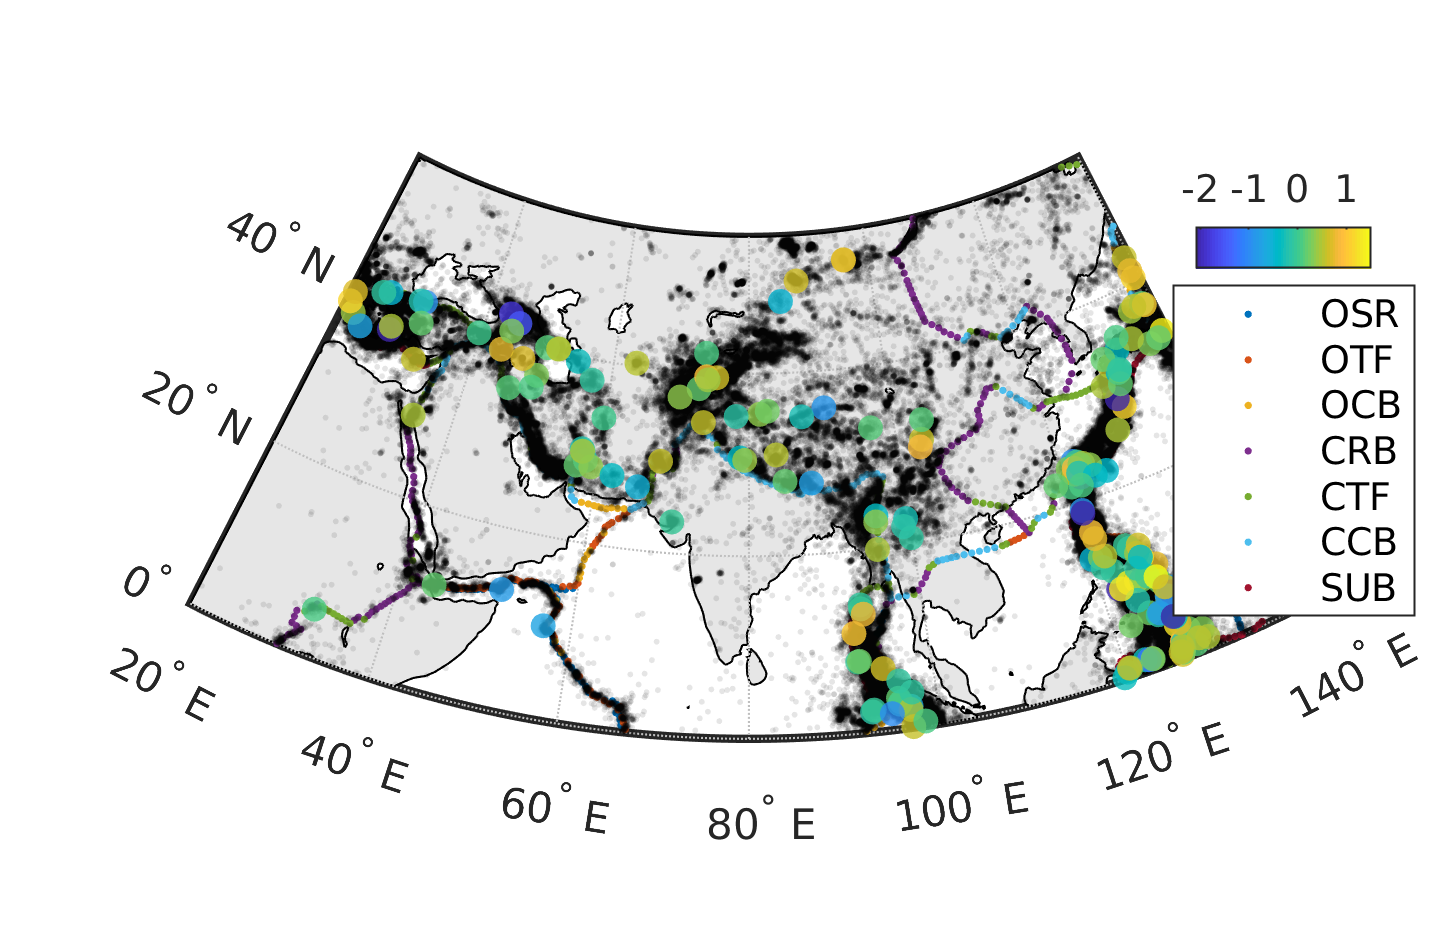
\includegraphics{figures/continental.png}
    \caption{Continental seismicity in Asia. Earthquake sequences (points) are colored according to their relative productivity. Note that as a general rule, continental earthquakes are well above the global average. Plate boundaries are abbreviated as follows: CCB continental convergent boundary, CTF continental transform fault, CRB continental rift boundary, OSR oceanic spreading ridge, OTF oceanic transform fault, OCB oceanic convergent boundary, SUB subduction zone.}
    \label{fig:continental}
\end{figure}

\begin{sidewaysfigure}[!p]
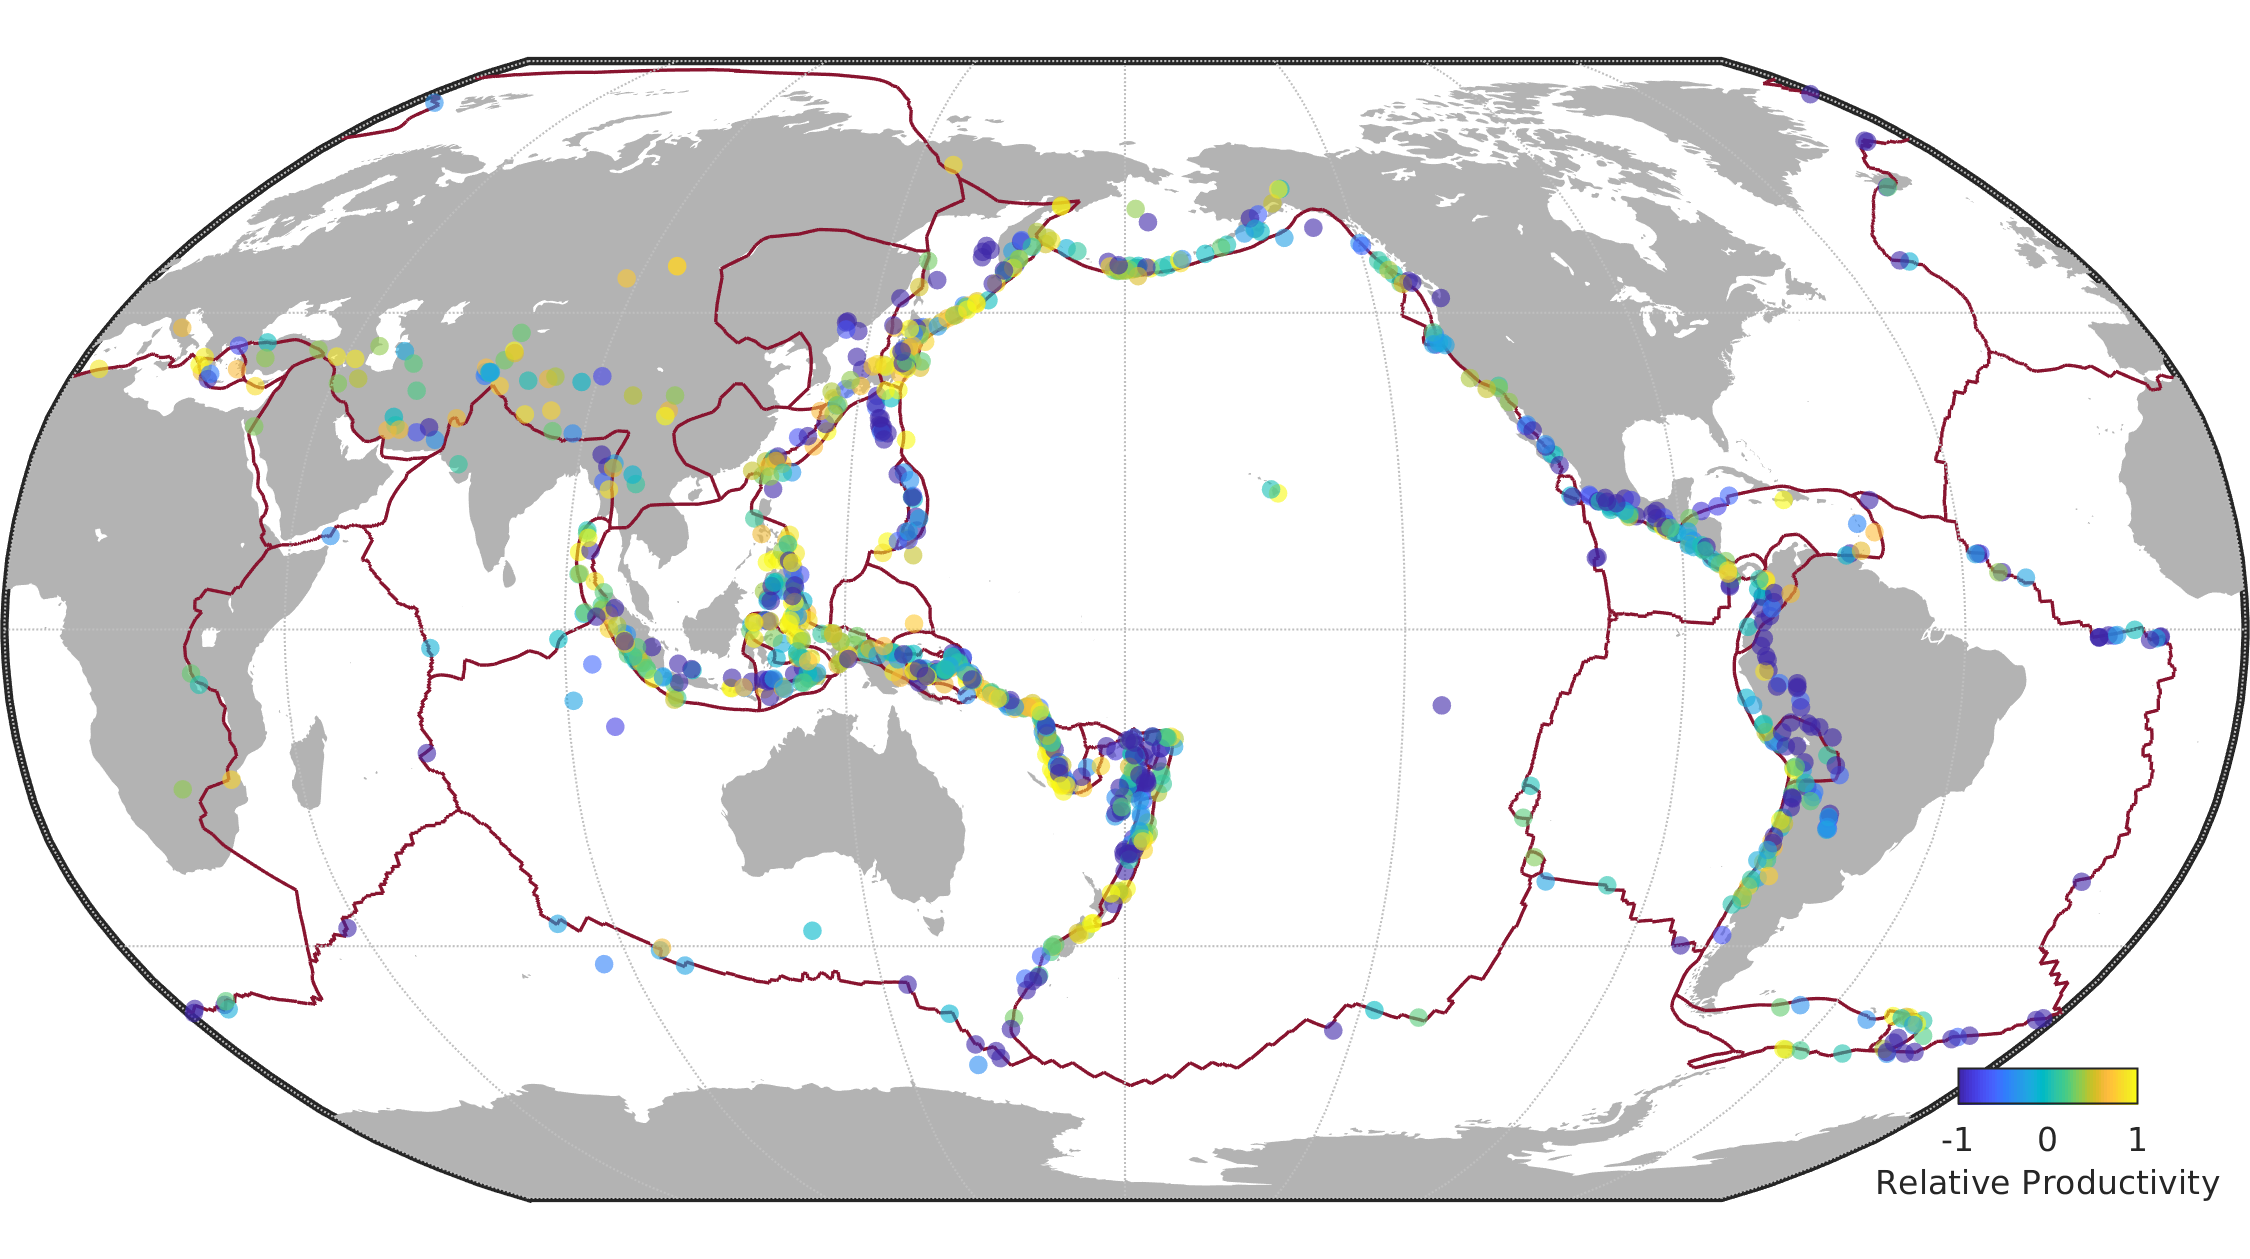
\includegraphics{figures/worldmap_res.png}
    \caption{Global map of earthquake productivity. Colored lines follow the surface trace of the tectonic boundaries. Black points indicate all earthquakes in the catalog. All mainshocks are color-coded according to their relative productivity ($N*$). Plate boundaries are abbreviated as follows: CCB continental convergent boundary, CTF continental transform fault, CRB continental rift boundary, OSR oceanic spreading ridge, OTF oceanic transform fault, OCB oceanic convergent boundary, SUB subduction zone} 
    \label{fig:global_res}
\end{sidewaysfigure}

\begin{figure}
    \centering
    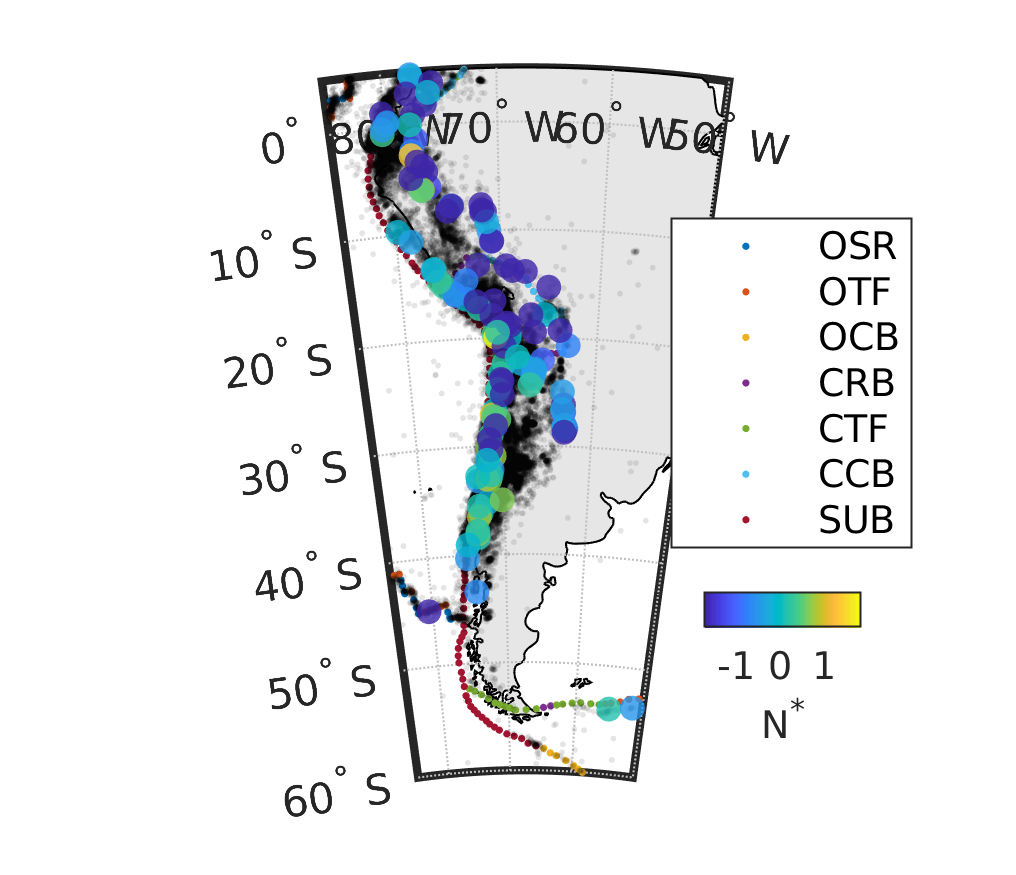
\includegraphics[]{figures/south_america.png}
    \caption{Regional pattern in aftershock productivity. Note the band of low productivity corresponding to deep focus earthquakes}
    \label{fig:atacama}
\end{figure}

\section{Tectonic setting}\label{sec:tectonic_setting}

Are strike-slip earthquakes deficient in aftershocks because of characteristic settings? In this section, we explore tectonic controls on the productivity of earthquake sequences.

We first tested this hypothesis by examining whether earthquakes with different focal mechanisms that share the same geographic location still exhibit statistically distinct earthquake productivity. If the tectonic setting is the only control on the relative productivity of earthquakes, then strike-slip earthquakes should not exhibit fewer aftershocks when controlling for the tectonic setting. 

We collected a catalog of co-located strike-slip and dip-slip earthquakes. We iteratively cataloged the nearest pair of strike-slip and dip-slip mainshocks taking care not to double count earthquakes in this process. The productivity of co-located strike-slip and dip-slip earthquakes generally correlate with each other (see figure \ref{fig:coloc}). The distinction by faulting style is not significant when comparing only co-located earthquakes (see Figure \ref{fig:nearSS}). This first step supports a tectonic control of the productivity of earthquakes and justifies further inquiry into the question.

\begin{figure}
    \centering
    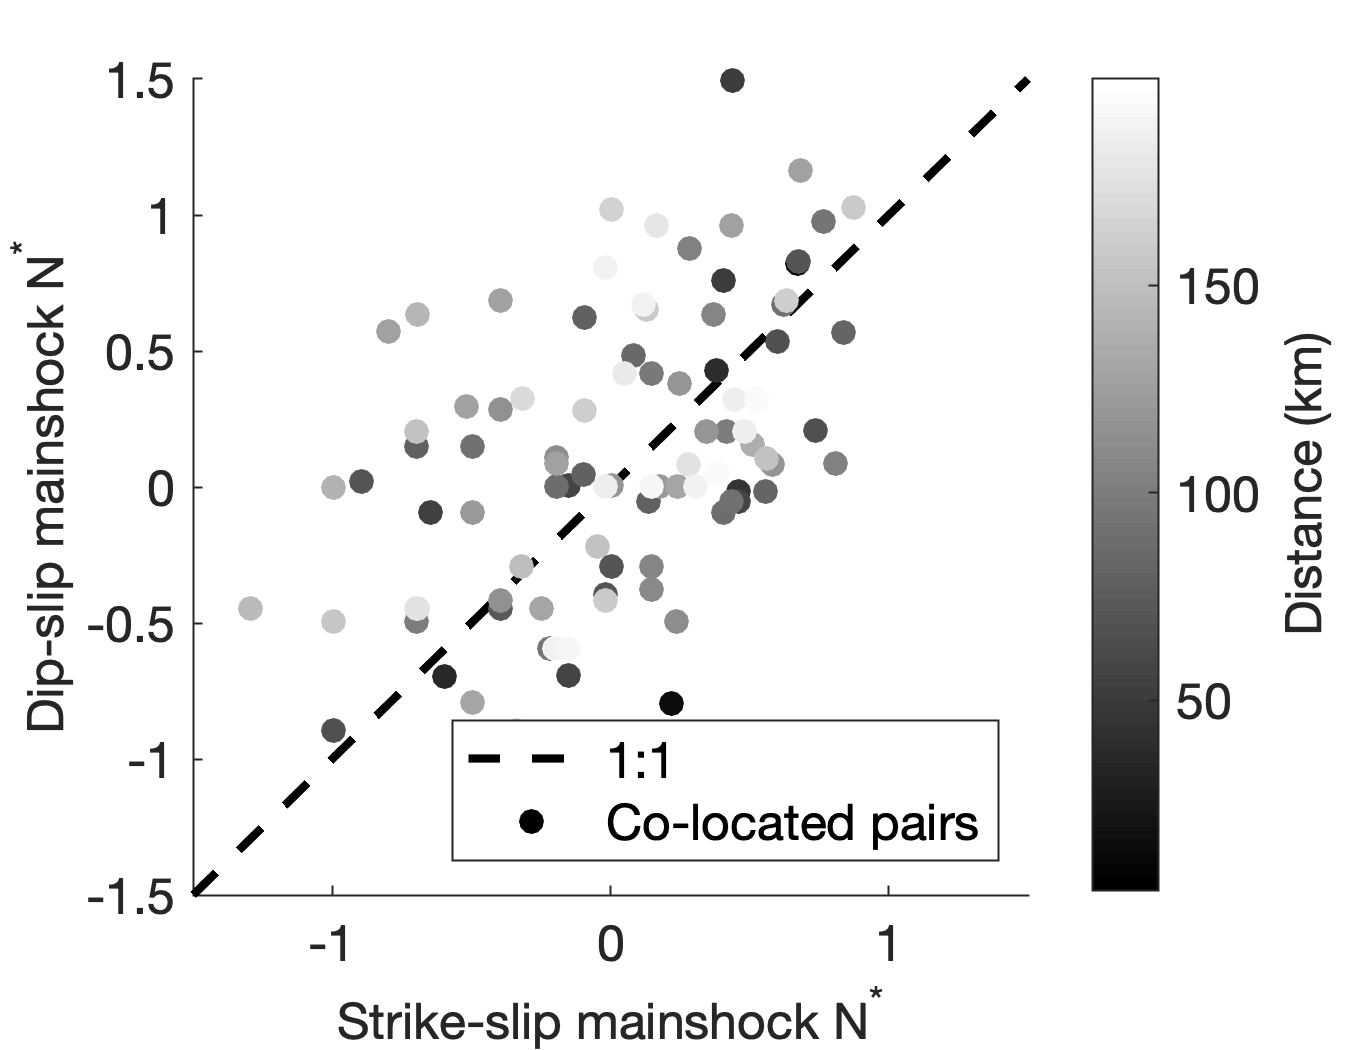
\includegraphics{figures/colocated_res.png}
    \caption{Relative aftershock productivity for corresponding pairs of earthquake sequences with strike-slip and dip-slip mainshocks with a mainshock larger than $M_w6.5$. Each pair is shaded according to their relative distance.}
    \label{fig:coloc}
\end{figure}

\begin{figure}
    \centering
    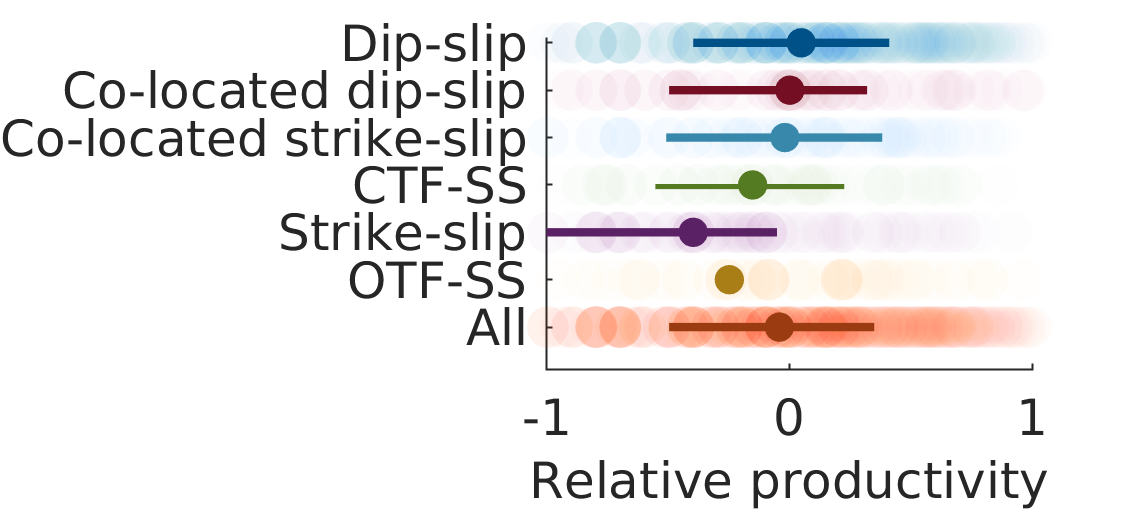
\includegraphics{figures/nearSS.png}
    \caption{Relative aftershock productivity for sequences with a mainshock larger than $M_w6.5$ across various subsets of the global catalog. Transparent points are individual sequences. Solid points are the median and interquartile range of the relative productivity measurements.  CTF-SS is short for strike-slip earthquakes on continental transform faults; OTF-SS is short for strike-slip earthquakes on oceanic transform faults. We draw particular attention to strike-slip earthquakes co-located on a pair-wise basis with dip-slip earthquakes. Note that these two subsets of the data are not significantly different (p = 0.63).}
    \label{fig:nearSS}
\end{figure}

We provide an overview of productivity by tectonic setting. We leverage the digitization of \textcite{Bird2003AnBoundaries} to categorize earthquake sequences by tectonic boundary (see Figure \ref{fig:plate_boundary}). Sequences were categorized according to the mainshock's distance to a digitized plate boundary and its focal mechanism. Based on this analysis, oceanic transform faults (OTF) are particularly deficient in aftershocks. Comparatively, continental transform faults (CTF), are more productive. Subduction zone (SUB), continental convergent boundaries (CCB), continental rift basins (CRB) and oceanic convergent boundaries (OCB) have similar and generally elevated relative productivity. It is difficult to assess how representative the productivity estimate for oceanic spreading ridges is given the small sample size of $M_w 6.5+$ earthquakes.

\begin{figure}
    \centering
    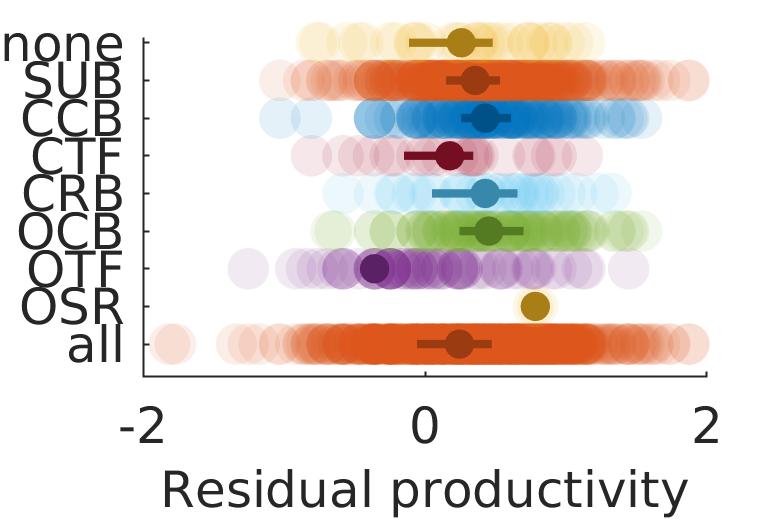
\includegraphics{figures/prod_by_plate_boundary.png}
    \caption{Earthquake productivity by tectonic boundary. Boundary types: None intraplate, CCB continental convergent boundary, CTF continental transform fault, CRB continental rift boundary, OSR oceanic spreading ridge, OTF oceanic transform fault, OCB oceanic convergent boundary, SUB subduction zone}
    \label{fig:plate_boundary}
\end{figure}

We alluded to a possible relationship between earthquake productivity and the age of the lithosphere. Here, we offer a quantitative assessment. We determined the age of the lithosphere hosting each mainshock using oceanic ages reported in \textcite{Muller2008}. We discarded earthquakes sequences for which the mainshock was more than 30 km from an estimate of oceanic lithosphere age. Accordingly, continental earthquakes were not included in the analysis. 

We find that earthquake sequences in younger oceanic lithosphere tend to have fewer aftershocks (see Figure \ref{fig:prod_vs_age}). Considering all mainshocks, we observe a more rapid change in productivity in the first $\sim 50$ Ma of the oceanic lithosphere which tapers away as the oceanic lithosphere ages. Earthquakes with no aftershocks are strongly biased to young ages. The general trend is repeated, though more scattered, for each faulting style in isolation.

\begin{figure}
    \centering
    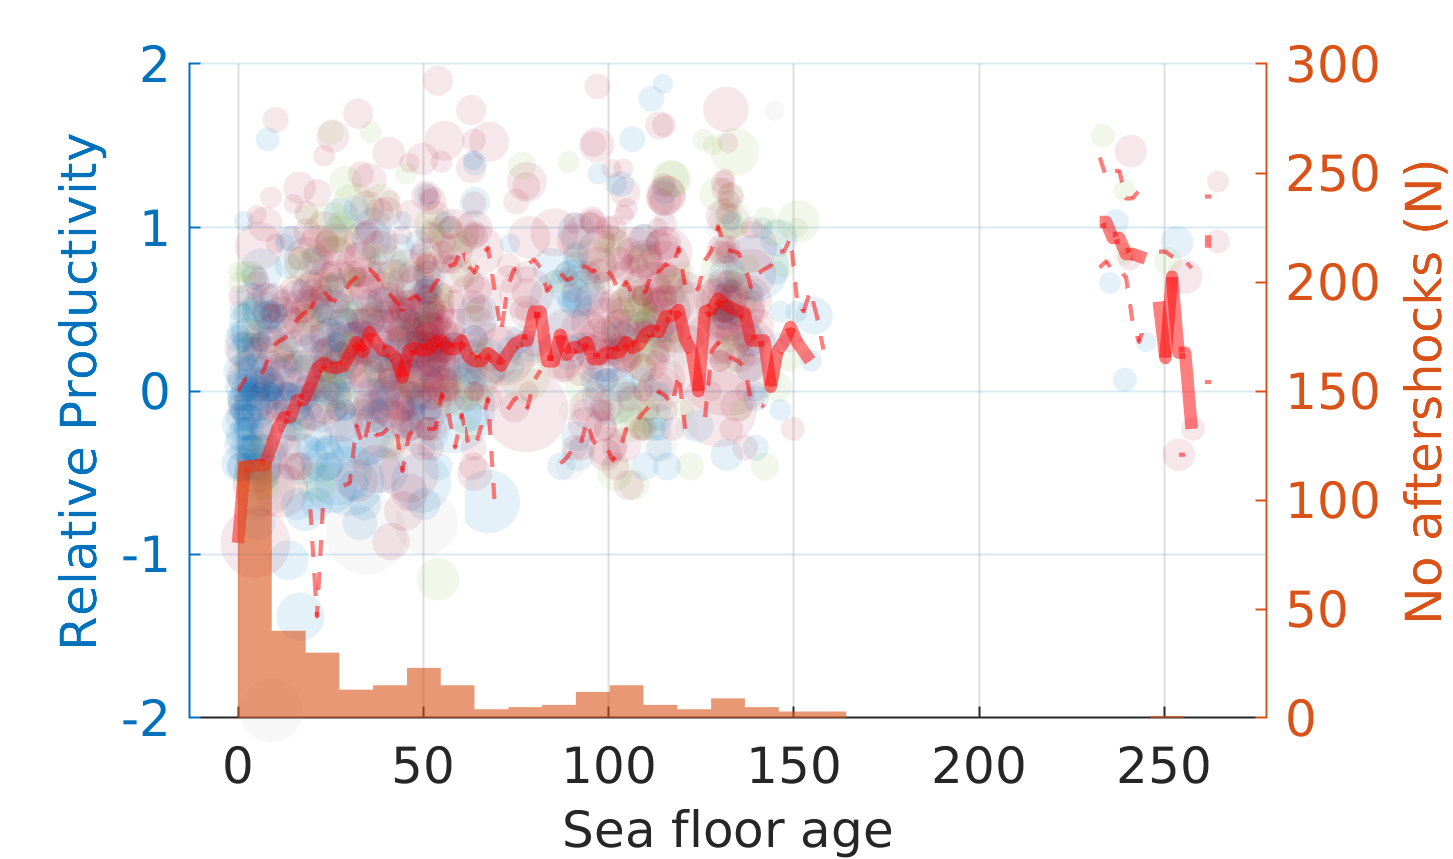
\includegraphics{figures/prod_vs_age.png}
    \caption{Relative productivity as a function of age of the oceanic lithosphere. Each point indicated an individual earthquake sequence. Sequences are color-coded according to faulting style of the mainshock (blue: strike-slip, green: normal and red: reverse). The red line is a moving median window. Dashed lines indicate the 33rd to 66th percentile range. Earthquakes with no aftershocks (binned by seafloor age) cannot be measured with relative productivity. Nonetheless, the moving median records these sequences.}
    \label{fig:prod_vs_age}
\end{figure}
which the mainshock was more than 30 km from an estimate of oceanic lithosphere age. Accordingly, continental earthquakes were not included in the analysis. 

We find that earthquake sequences in younger oceanic lithosphere tend to have fewer aftershocks (see Figure \ref{fig:prod_vs_age}). Considering all mainshocks, we observe a more rapid change in productivity in the first $\sim 50$ Ma of the oceanic lithosphere which tapers away as the oceanic lithosphere ages. Earthquakes with no aftershocks are strongly biased to young ages. The general trend is repeated, though more scattered, for each faulting style in isolation.

\section{Source parameters}\label{sec:source_parameters}

Are strike-slip earthquakes deficient in aftershocks because of characteristics of the source? In this section, we test whether there exists source attributes that are characteristic of strike-slip earthquakes that may cause them to have fewer aftershocks. 

We first assemble a comprehensive set of source parameters paying particular attention to characteristic features of strike-slip earthquakes and any other parameters likely to affect the productivity of earthquakes.

\subsection{Analyzed parameters}

\subsubsection{Radiated energy}
\textcite{Convers2011GlobalMid2010} cataloged the radiated energy of global earthquakes with earthquake magnitudes exceeding M7. The radiated energy is estimated from the p-wave velocity spectrograms of teleseismic stations. The radiated energy is a natural feature to analyze given mounting evidence for dynamically triggered aftershocks \cite{Brodsky2011TheForeshocks,felzer2006decay}. We obtain a catalog of radiated energy from the IRIS data management services. The catalog also contains estimates of rupture duration which we also include in the analysis.

\subsubsection{Source dimensions}
\textcite{Hayes2017} has assembled a catalog of finite fault inversions for all great earthquakes from 1990 to present (2018). The catalog was produced under a self-consistent processing scheme. The finite fault inversions, provide the spatial distribution of slip as inverted from teleseismic stations. Slip is discretized onto sub-faults with dimensions on the order of kilometers. From the finite fault inversion, following \textcite{MartinMai2000}, we recover the width (along-dip) and length (along-strike) of the rupture using the autocorrelation width:

\begin{equation}
    W = \dfrac{\int_{-\infty}^{\infty} (f*f)dx}{f*f|_{x=0}}.
\end{equation}

where $W$ is the autocorrelation width of the cumulative slip function $f$ along the direction $x$. The auto-correlation regularizes slip distributions and circumvents the issue of choosing an arbitrary slip contour as the edge of the rupture. From the estimates of width and length, we also record the aspect ratio of each rupture.

To parameterize the complexity of each rupture, we devised a measure of slip heterogeneity. Our measure differentiates the actual slip distribution from a reference `idealized' positive ellipsoidal slip distribution.
%
\begin{equation}
    H = \int_\Sigma (u-u_{ref})^2 dS,
\end{equation}
%
\begin{equation}    
    \dfrac{u_{ref}^2}{u_{max}} + \dfrac{(x-x_0)^2}{a^2} +   \dfrac{(y-y_0)^2}{b^2} = 0,
\end{equation}
where $u$ is the slip distribution, $u_{ref}$ is the reference slip distribution implicitly defined by parameters $u_{max}, x_0, y_0, a$ and $b$ which are fit to the actual slip distribution.

\subsubsection{Stress drop}

We measure stress drop for each rupture from finite fault inversions. Global compilations derive stress drop estimates from corner frequencies \cite{Allmann2009GlobalEarthquakes}. We prefer to produce new estimates of stress drop that do not rely heavily on assumptions of uniform source dimensions, shape and rupture velocity times. Each of these assumptions may affect aftershock productivity. We follow recommendations from  \textcite{Noda2013} and allow stress drop measurements account for heterogeneous slip. The stress drop estimation ($\bar{\Delta \sigma_E}$) leverages energy considerations whereby:
\begin{equation}
    \bar{\Delta \sigma_E} = \dfrac{\int_\Sigma \Delta \boldsymbol{\sigma}\cdot \Delta \boldsymbol{u} dS}{\int_\Sigma \Delta u_1 dS},
\end{equation}
where $\Delta \boldsymbol{\sigma} = \tau^{ini}-\tau^{fin}$ is the change in shear stress at a point, $\Delta \boldsymbol{u}$ is the slip on the fault. We derive the change in stress at any given point of the fault and the stress drop $\bar{\Delta \sigma_E}$ from the finite fault inversions from the \textcite{Hayes2017} catalog.

Smoothing constraints on the finite fault inversions imply that the stress drop measurements are likely a lower bound \cite{Adams2017ExploringInversions}. Nonetheless, these estimates should be more robust than others \cite{Noda2013}. Estimation of stress drop, $\Delta \sigma_E$, for complex ruptures with multiple oblique fault planes is not yet developed. A thorough treatment of the physics involved and the implementation thereof in this analysis is currently beyond the scope of this work. As a consequence, we only retain 98 ruptures for the subsequent analysis. I will address this issue in future work.

\subsection{Results}

The number of parameters of potential significance involved in the \textcite{Hayes2017} catalog renders a parameter-by-parameter analysis cumbersome. To highlight variables to that may be relevant to our analysis, we regress each available parameter to the relative productivity. To assess the significance of each fit, we report the goodness of fit ($R^2$) and compare it to 10000 Monte Carlos simulation of the same catalog, only shuffled at each iteration.

An analysis of linear relationships between individual earthquake parameters and relative productivity (see figures \ref{fig:Energy}-\ref{fig:aspect}) reveals some significant features. Before addressing relationships that do appear to relate to productivity, we consider radiated energy and scaled duration as examples of null results. While there is a separation by focal mechanism, there does not appear to be any trend across the entire data set. 

The scaled energy, scaled length, Poisson's Ratio, heterogeneity, Young's Modulus, and Rupture velocity do not yield statistically significant linear regressions with relative productivity. 
 
Our analysis suggest the stress drop and aspect ratio are the only parameters to yield statistically significant regressions. On average, low aftershock productivity is associated to low stress drop and high aspect ratio. 

\begin{figure}[!ht]
    \centering
    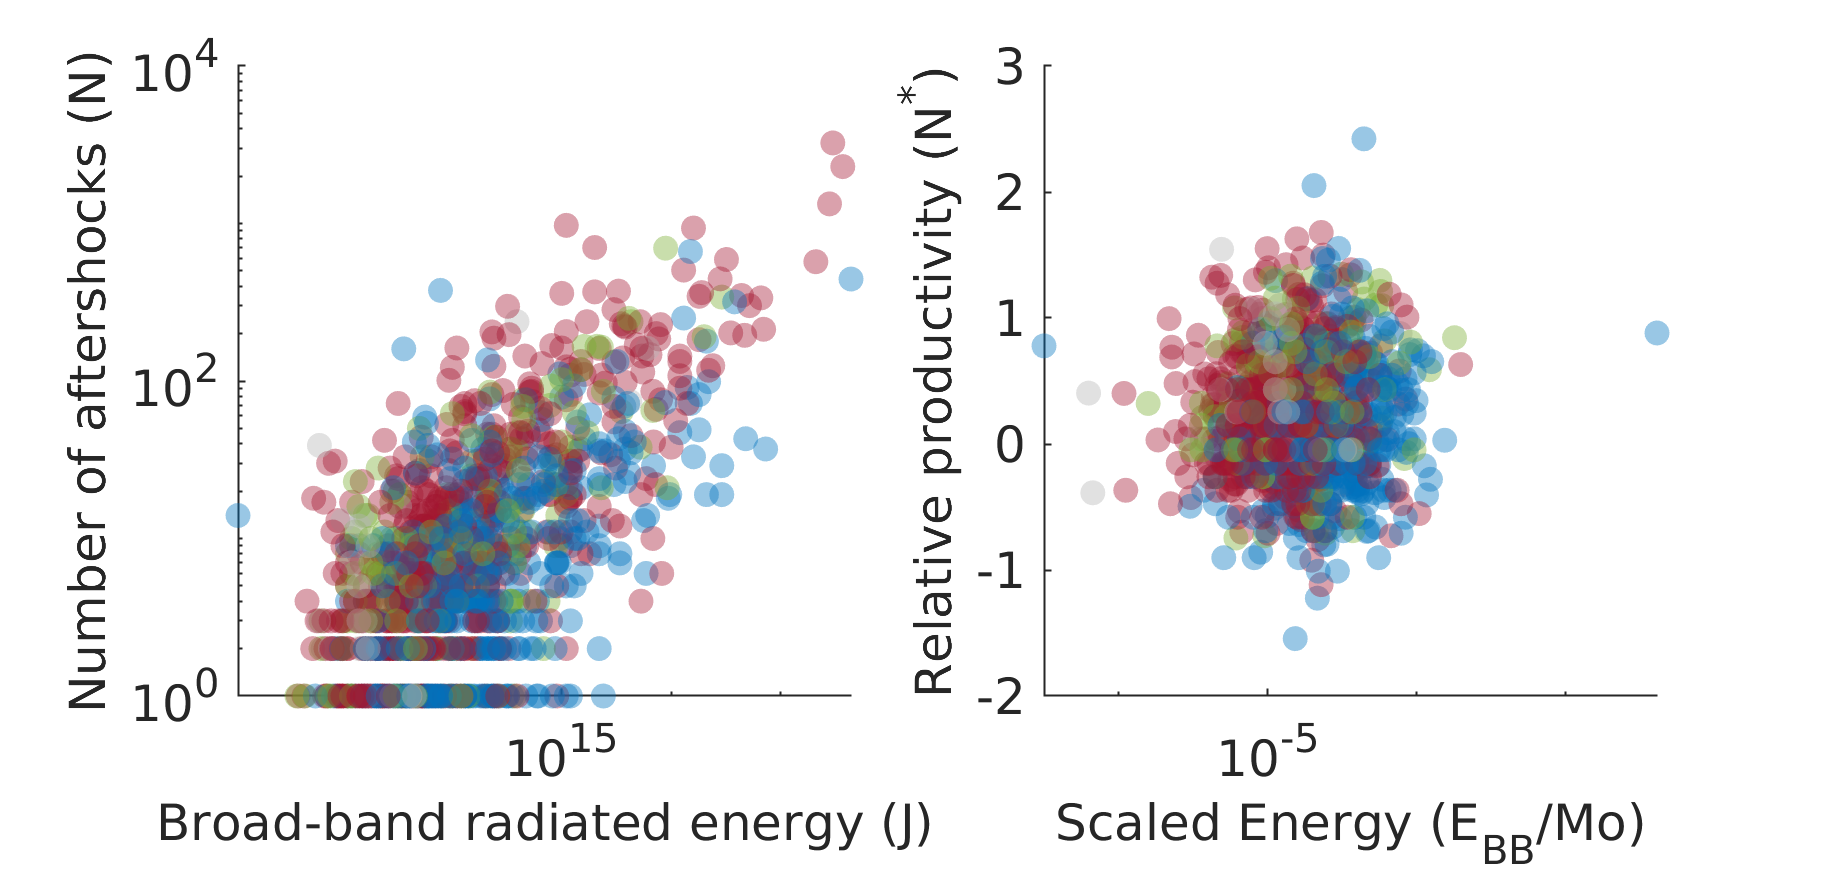
\includegraphics{figures/prod_vs_energy.png}
    \caption{Left: Number of aftershocks as a function radiated energy. Right: relative productivity as a function of scaled earthquake energy ($E_{BB}/M_0$). The scaled earthquake energy removes any magnitude dependence to the radiated energy. Note that while the radiated energy appears to cluster focal mechanisms more tightly than in the original productivity law, there is no clear trend in the entire dataset relating radiated energy to relative productivity. Sequences are color-coded according to the faulting style of the mainshock (blue: strike-slip, green: normal and red: reverse).}
    \label{fig:Energy}
\end{figure}

\begin{figure}
    \centering
    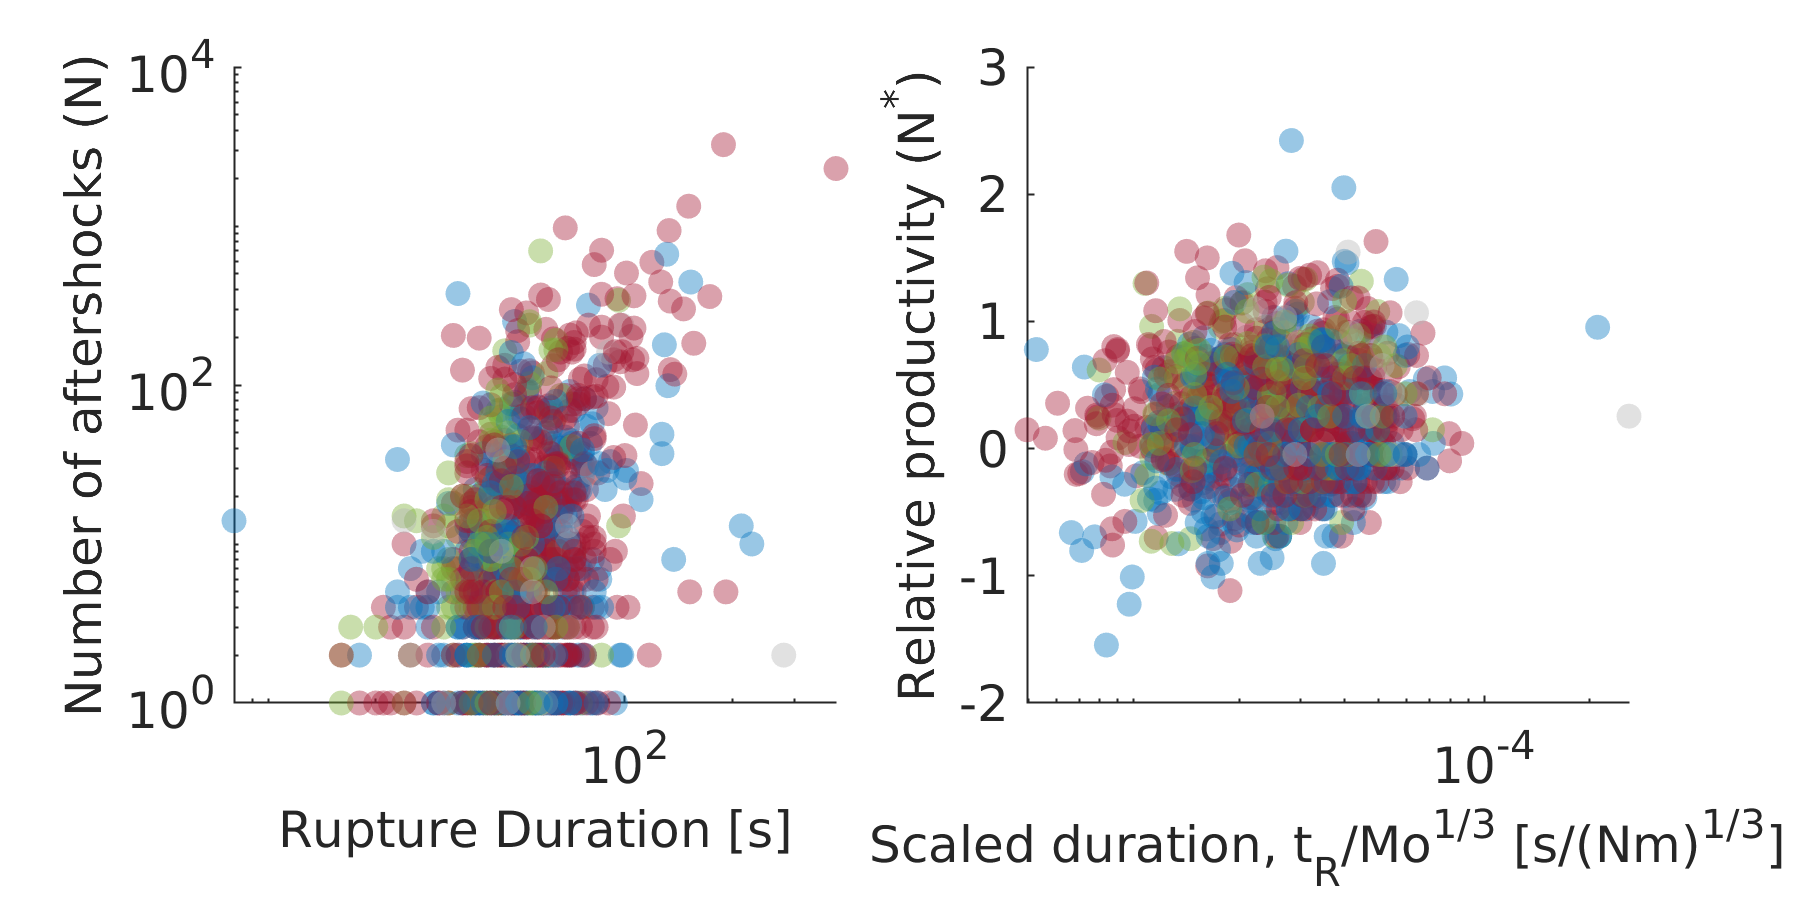
\includegraphics{figures/prod_vs_dur.png}
    \caption{Left: Number of aftershocks as a function rupture duration. Right: relative productivity as a function of scaled rupture duration ($t_R/{M_0}^{1/3}$). There is no clear trend in the entire dataset relating rupture duration to relative productivity. Sequences are color coded according to faulting style of the mainshock (blue: strike-slip, green: normal and red: reverse).}
    \label{fig:prod_vs_dur}
\end{figure}

\begin{figure}
    \centering
    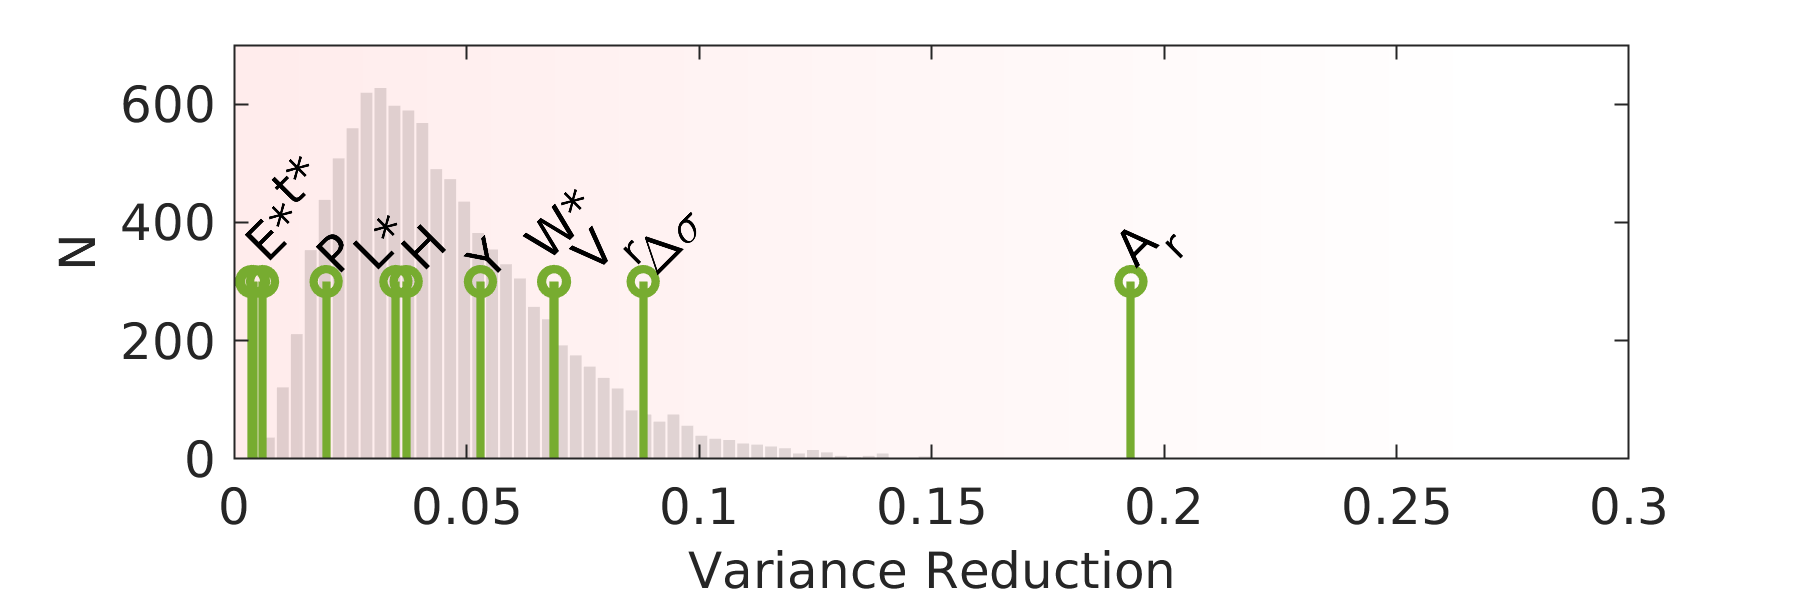
\includegraphics{figures/r2stems.png}
    \caption{Goodness of fit of linear regressions for each source attribute in our catalog. The scaled energy ($E*$), scaled length ($L*$), Poisson's Ratio ($P$), heterogeneity (H), Young's Modulus (Y), Rupture velocity (V) all do not achieve a statistically significant fit to the relative productivity. The stress drop $\Delta \sigma$ and, by a large margin, the aspect ratio ($A_r$) of the rupture yield the best fitting linear regressions.}
    \label{fig:r2_finite_fault}
\end{figure}

\begin{figure}
    \centering
    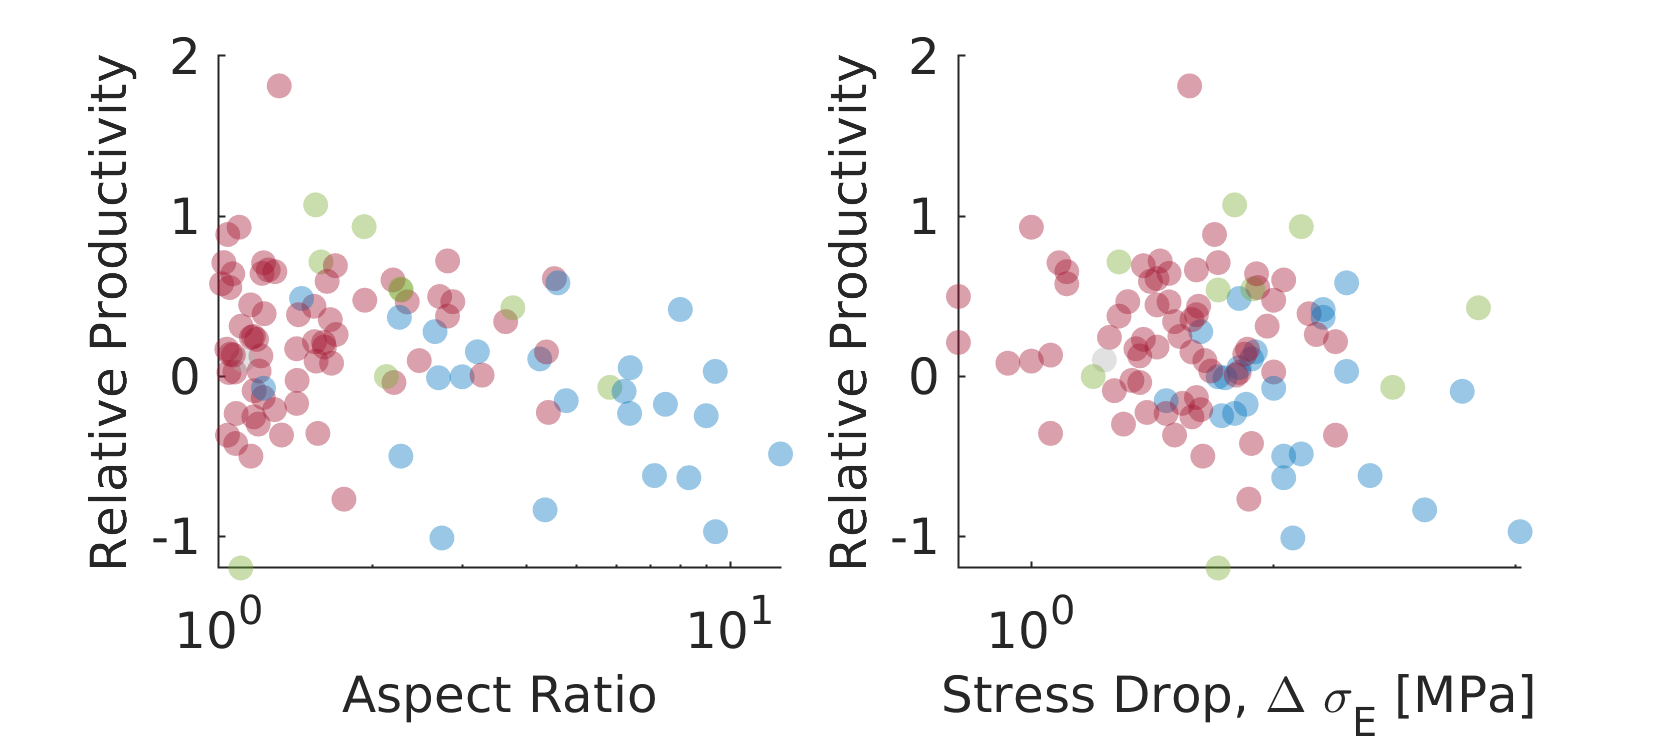
\includegraphics{figures/prod_vs_aspect.png}
    \caption{Left: Relative earthuqake productivity as a function of mainshock aspect ratio as determined from auto-correlation widths and lengths of finite fault inversions\cite{Hayes2017}. Right: Relative productivity as a function of recomputed stress drops ($\Delta \sigma_E$) determined directly from finite fault inversions}
    \label{fig:aspect}
\end{figure}

\section{Discussion}

% current outline:

% recap: 
%   deep earthquakes
%   continental earthquakes
%   plate age

% interp and discussion of plate age

% source attributes recap
%   energy
%   stress drop
%   missing heterogeneity
%   aspect ratio

% literature context?

% multi attribute ML

% conclusion



\subsection{Significant results}

The description of the global map of productivity highlighted that 1) deep-focus earthquakes generate fewer aftershocks than do shallow earthquakes, 2) plate boundary and continental earthquakes differ starkly, 3) aftershock productivity appears to correspond to the age of the oceanic lithosphere. Our quantitative analysis supports these observations. 

We find clear distinctions between shallow and deep seismicity. There is a large body of literature examining the distinct earthquake statistic associated with deep earthquakes. Low aftershock productivity is a known feature of deep earthquakes and is generally attributed to the temperature of the downgoing slab. A large body of literature has documented this observation in the global catalog \cite{Bath1965LateralMantle, Frohlich1987AftershocksEarthquakes,Nyffenegger2000} and regionally \cite{Wiens1997AftershockZone, Wu1999}. The exact cause of the deficiency in aftershocks is contentious \cite{Nyffenegger2000}.

We show that different tectonic environment have distinct signatures in aftershock productivity. Observations of elevated productivity for continental earthquake date back to \cite{Mogi1967EarthquakesFractures, Davis1991Single-linkVariations}. This observation is in general agreement of \textcite{Page} who evaluated global productivity and Bath's law parameters for different tectonic settings and found that active non-subduction continental regions generally have elevated earthquake productivity and, on average, larger aftershocks. There is a good reason to differentiate oceanic and continental plate boundaries. We expect the mechanical system within tectonic plates to be far less mature and more diffuse. Scaling laws often differentiate between the plate boundary and intraplate earthquake \cite{Scholz2019TheFaulting}. 


We found a secular increase in earthquake productivity with plate age. To our knowledge, a relationship between aftershock productivity and plate age of the oceanic lithosphere is a new finding. Before we interpret this result, we assess whether this result may arise from catalog artifact. Mid-ocean ridges are especially challenging to instrument. Whether or not we observe fewer aftershocks because of sparse instrumentation in these regions is a reasonable concern. The same analysis with a more conservative completeness of $M_w5$ yields the same general trend.

This result may explain many patterns in aftershock productivity. The elevated productivity of the Mediterranean sea which has some of the oldest oceanic lithospheres on Earth is highly productive (see Figure \ref{fig:global_res} for reference). The relative productivity tracks a square root conductive cooling of the oceanic lithosphere. A cool oceanic lithosphere is more brittle, less buoyant and thicker. There is some evidence to show that earthquake statistic could track lithospheric cooling \cite{Bird2003AnBoundaries, Bird2004Plate-TectonicSettings,Nishikawa2014EarthquakeBuoyancy}. Subduction zone earthquakes hosted along younger lithosphere tend to generate larger earthquakes (lower b-values), particularly so in the first $\sim70$ Ma.  \textcite{Nishikawa2014EarthquakeBuoyancy} attribute the trend to changes in buoyancy of the subducting slab. We find it difficult to reconcile their penultimate interpretation with our observations.  How buoyancy would directly affect seismicity along transform fault is unclear. The exact coupling of b-value statistics and earthquake productivity certainly deserves to be further explored. Alternatively, an older and therefore thicker brittle oceanic lithosphere could promote aftershocks by increasing the availability of critically stressed faults. 

We emphasize that this result transcends faulting styles. Subduction zones also share this pattern \cite{Wetzler2016}. Conversely, a large portion of global strike-slip mainshocks is hosted in young oceanic lithosphere along transform faults which may explain why, on average, strike-slip earthquakes have fewer aftershocks. 

If we extend this interpretation a step further, we may cast continental earthquakes as a highly thickened (old) lithosphere end member; conversely, we may view deep focus earthquakes as `rejuvenated' oceanic lithosphere caused to thin by thermal conduction from the warmer mantle. 

Our observations seem to indicate that the tectonic setting matters. When carefully removing any possible effect from a spatially uneven sampling of different tectonic settings, we found no significant difference between faulting style. It is difficult to construe confounding effects causing only strike-slip earthquakes located near corresponding dip-slip mainshocks to be more productive. In short, a first-order explanation to the question motivating this research: \textit{Why do strike-slip earthquakes generate fewer aftershocks?} Strike-slip earthquakes are typically in environments that generate fewer aftershocks.

Our analysis of the finite inversions for large earthquake ruptures highlighted a significant relationship between the productivity of an earthquake and source attributes. Below, we discuss significant results:

\textit{Earthquake energy:} If dynamic triggering dominates the production of aftershocks, The energy radiated away from a mainshock scaled by the moment of the mainshock would be expected to trigger more earthquakes should dynamic triggering dominate the production of aftershocks. Strike-slip earthquakes radiate more energy when controlling for magnitude. However, our result shows no correlation with the scaled radiated energy of the mainshock. This result suggests that within a few source dimensions of the mainshock static and quasi-static effect dominate earthquake triggering processes. It might be interesting to further investigate the far-field aftershock productivity (e.g., teleseismic triggering) and see whether the absence of correlation with radiated energy persists.

\textit{Slip heterogeneity:} A long-standing contention is that the productivity of aftershocks is related to the heterogeneity of the fault system \cite{Mogi1967EarthquakesFractures, Utsu1995}. To parameterize heterogeneity, we measured the irregularity of the slip distribution relative to the idealized slip distribution. Mainshocks with irregular slip do not have more aftershocks. We might have expected more heterogeneous ruptures to have more aftershock because in-plane aftershocks often delineate areas of irregular slip \cite{Yabe2018}, the observation may suggest that the aftershocks in the surrounding volume dominate the count \cite[consistent with][]{Wetzler2018SystematicEarthquakes}.

\textit{Stress Drop:} Higher stress drop marginally correlates with lower aftershock productivity. \textcite{Wetzler2016} noted the same result for great subduction zone earthquakes. The authors interpreted the seemingly perverse result as the trade-off between source dimensions and slip on the fault. Accordingly, for fixed magnitude, earthquakes with higher stress drops have a smaller source dimension, activate a smaller volume and trigger fewer aftershocks. In the competition between the intensity of the stress of the earthquake and the volume of the earth's crust that is activated, the geometric effect dominates \cite{Wetzler2016}. 

\textit{Aspect Ratio:} Ruptures with longer aspect ratios tend to have fewer aftershocks. Long aspect ratio ruptures reflect the saturation of the brittle crust--- above by the surface of the Earth and below by viscous dissipation. We expect the confines of the brittle crust to limit the productivity of aftershocks. The spatial confines limit the volume that may host aftershock. It is telling to observe that while both are not significant, the down-dip width of the rupture correlates far better than the length of the rupture (as was shown in Figure \ref{fig:r2_finite_fault}). Vertical confines (the surface and the ductile base of the seismogenic zone) are far better controls on the productivity of earthquakes than the lateral limits. The inference may further help narrow our interpretation of the relationship between lithosphere age and earthquake productivity to a spatial effect. We expect younger lithosphere to be thinner, host longer aspect ratio ruptures and produces fewer aftershocks. 

\subsection{A multi-attribute prediction of aftershock productivity}

Short term hazard assessment relies on regional catalogs to calibrate the statistical behavior of the seismicity. Our analysis raises an exciting possibility. We have shown that parameters that have no memory of the local seismicity know about the upcoming seismicity of the aftershock. Teleseismic data and knowledge of the local tectonic context may determine short-term hazard following large earthquakes, notably, in historically poorly instrumented areas. Below we show how such a multivariate analysis could be conducted. 

In an exercise of synthesis, we tabulated earthquakes for which all parameters which we found to be significant exist. We include plate age, aspect ratio, stress drop, depth along with information about faulting style (dip and rake). Using all parameters causes over-fitting. Support Vector Machines (SVM) yielded the best predictions. Quadratic of cubic kernels yielded similar results. Support vector machines aim to find lines (in two dimensions), planes (in three dimensions), or hyper planes (in higher dimensions), that maximizes the margins of the data by mapping the data to higher dimensional spaces with transformations called kernels. SVMs are highly robust to over-fitting data and are therefore well suited for small datasets \cite{Witten2016DataTechniques}. The best predictions arose from the following inputs: a variant on the stress drop (scaled rupture area), fault dip and plate age (see figure \ref{fig:plotmatrix} for an overview of the co-variance matrix). \textcite{Wetzler2016} interpreted higher stress drops to correlate with lower productivity of a geometric effect. Earthquakes with high stress drop rupture on a smaller fault for a given magnitude \cite{Scholz2019TheFaulting}. To more directly measure the geometric effect, we included the normalized rupture area, $A_{norm} = \log{\dfrac{LW}{10^{-2.44+0.59M_w}}}$. Making plate age available to the learning exercise reduces the number of earthquakes available to the analysis. To avoid over-fitting the data, we perform 5-fold cross-validation. The cross-validation scheme iteratively sub-samples 4/5 of the data and generates a prediction for the remaining 1/5 of the data \cite{Witten2016DataTechniques}. The validation of the trained model is shown in figure \ref{fig:response}. The result has a root mean squared error of 0.3, is remarkably good given uncertainties involved in measuring the relative productivity.

\begin{figure}
    \centering
    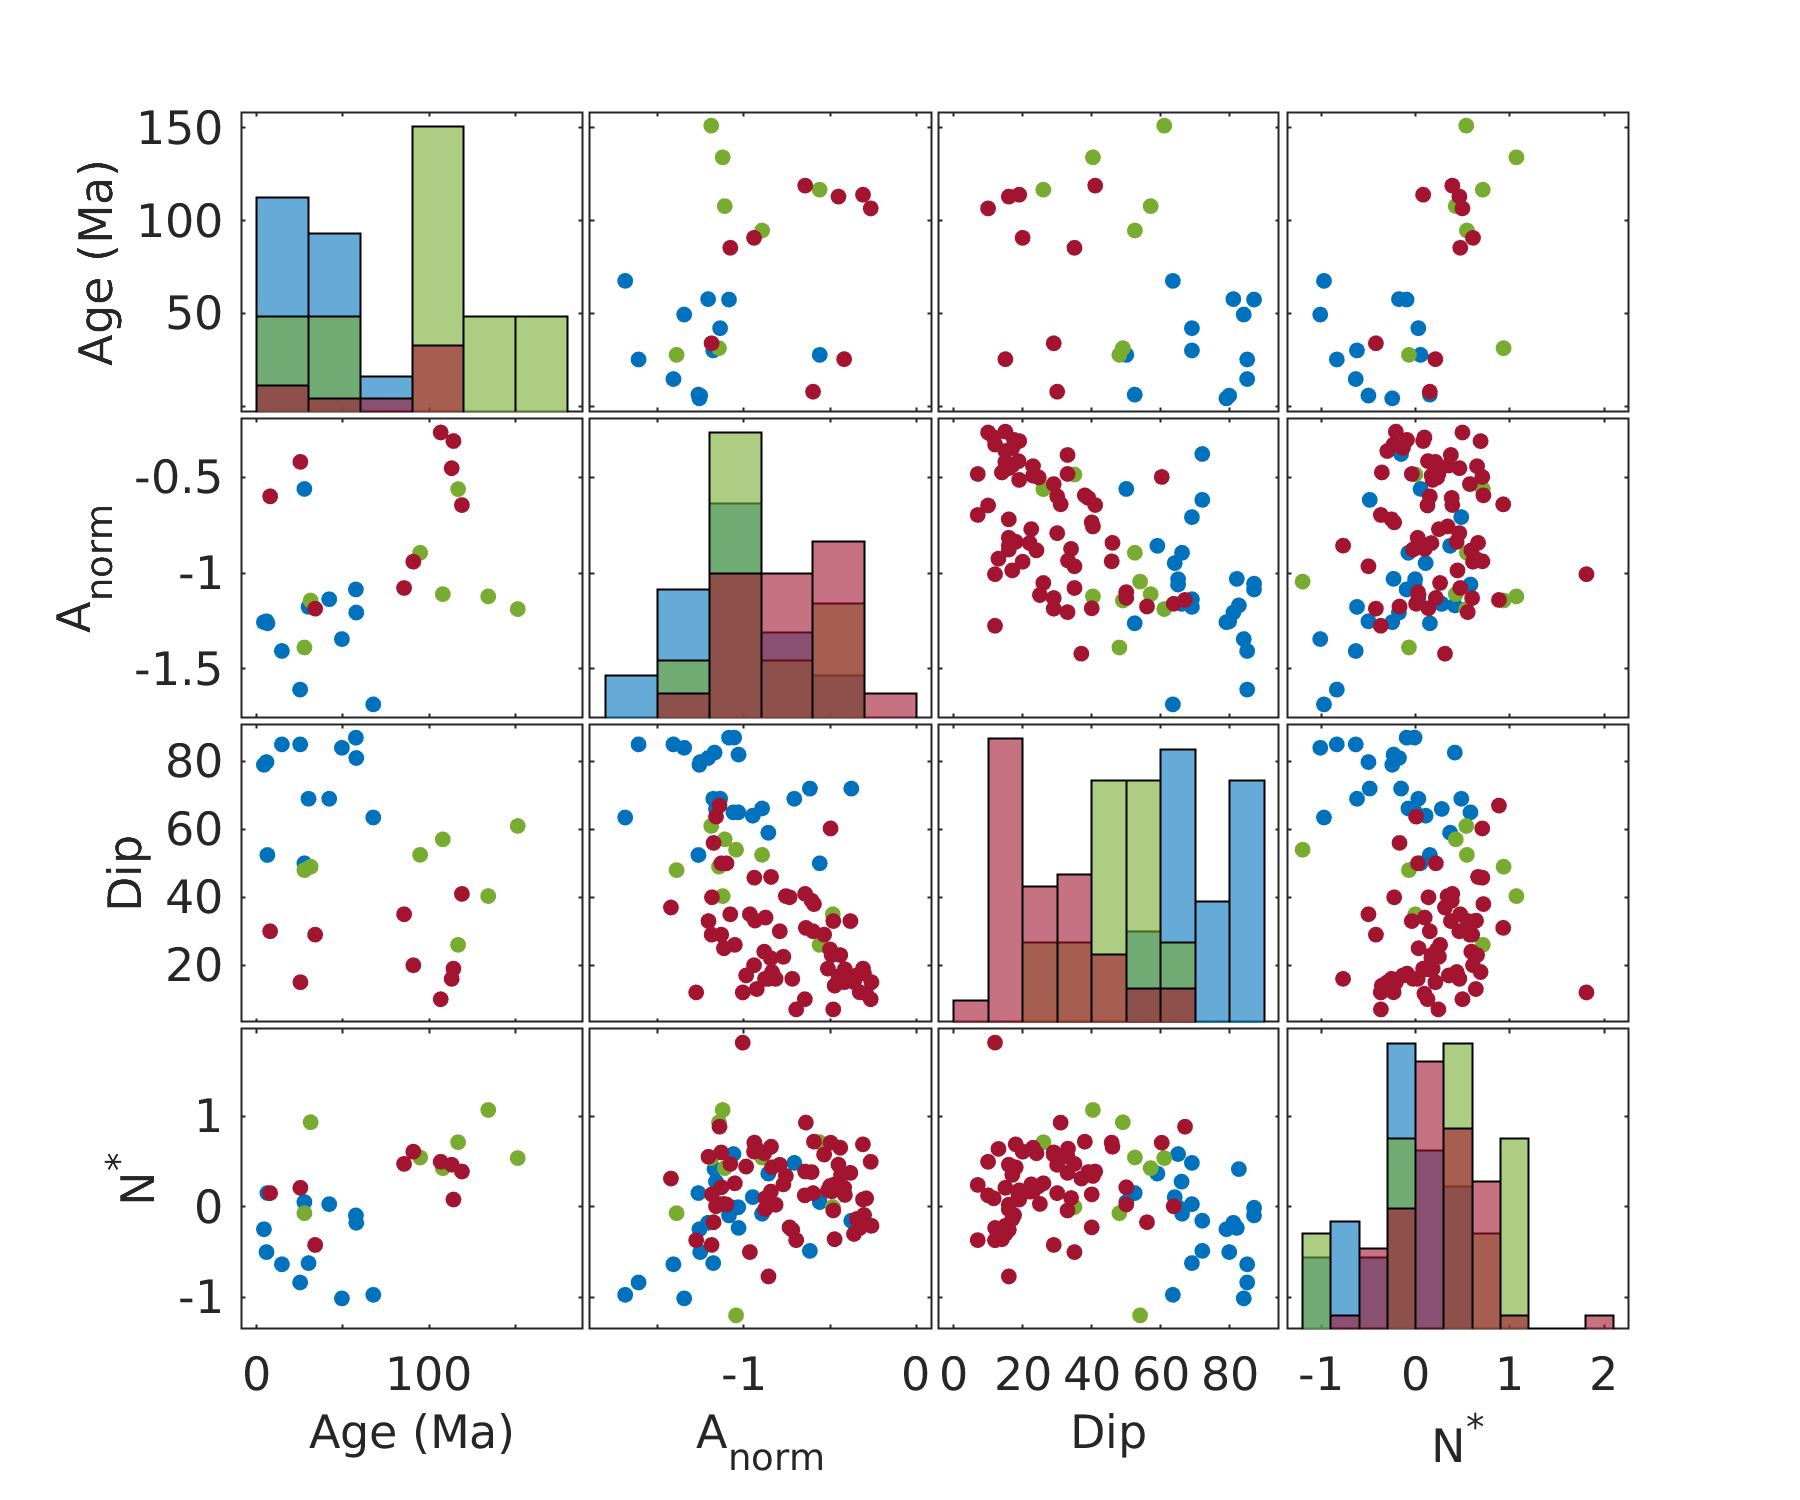
\includegraphics{figures/plotmatrix.png}
    \caption{Plot matrix of the selected parameters with respect to relative productivity, $N^*$ (grey background) and with eachother (white background). Mainshock sequences are colorcoded by focal mechanism type (blue: strike-slip, green: normal and red:reverse). Diagonal elements show the distribution of each parameter by focal mechanism following the same color scheme.}
    \label{fig:plotmatrix}
\end{figure}


\begin{figure}
    \centering
    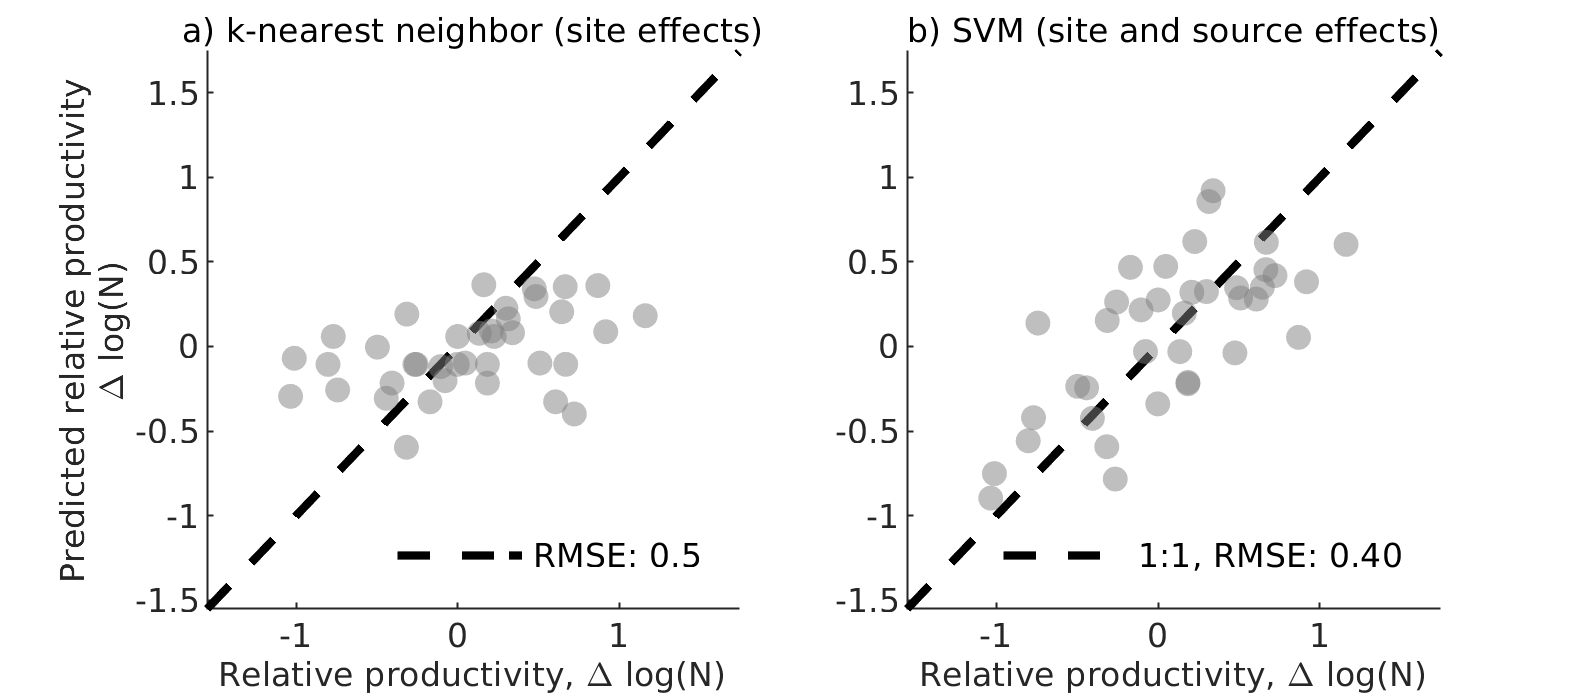
\includegraphics{figures/response.png}
    \caption{Response plot of the output of the trained model. Each point is an individual earthquake sequence color-coded by faulting style (blue: strike-slip, green: normal, and red: reverse). Note the good agreement between model predictions and actual values of relative productivity. A perfect prediction would set all values along the 1:1 line. Note that the model cleanly separates faulting style but also reveal trends within each faulting style group.}
    \label{fig:response}
\end{figure}

Various permutations of the data were selected in the process of producing the final trained model. It is curious that parameters such as aspect ratio, stress drop, rake, and depth did not yield improved models. We note that the final list of parameters (plate age, normalized area, and dip) are most directly related to the source geometry in space relative to the confines of the lithosphere. For instance, we found that the dip of the rupture is a better predictor than the rake of the rupture implying that the paucity in aftershocks may be less strongly modulated by the direction of rupture. The distillation of our input parameters also likely suggests some redundancy among them. Significant parameters found in section \ref{sec:source_parameters} may be symptomatic of the same source physics.

\section{Conclusion}

We found a paucity of aftershocks for strike-slip earthquakes relative to other focal mechanisms. Under careful examination, strike-slip earthquakes co-located with dip-slip earthquakes have similar aftershock productivity suggesting that the setting imparts control on the productivity of earthquakes. Global patterns suggest that earthquake productivity tracks lithospheric ages. The functional relationship suggests that productivity may increase because of the cooling and thickening of the oceanic lithosphere with time. 

We also correlated source parameters to the relative productivity of the corresponding aftershock sequence. Aspect ratio (log transformed) and, to a lesser degree, stress drop (log-transformed), linearly correlated with aftershock productivity; other parameters including rupture duration, normalized width, and length, scaled radiated energy and material parameters did not. Our observations reinforce that source geometry, and the availability of stressed faults exerts a first-order control on the number of aftershocks triggered. Particularly, we reveal the effect that the confines of lithosphere have on the availability of faults.

In a synthesis of our result, we find that just a few parameters (plate age, dip, and normalized rupture area) behold promising short-term predictive value. We emphasize that this prediction has no knowledge of the regional seismicity and therefore lends itself particularly well to large remote earthquakes where teleseismic data is available, but long term monitoring is not.


%%%%%%%%%%%%%%%%%%%%%%%%%%%%%%%%%%%%%%%%%%%%%%%%%%%%%%%%%%%%%%%%%%%%%%%%

\chapter{Large-scale detection of fault damage}\label{cpt:damage}

\begin{abstract}

Fault damage zones are inherently difficult to measure, yet determining their presence and size is critical to understanding earthquake mechanics. I will develop tools to couple remote observations of the Earth's topography to deep-seated physical features of a crustal fault damage zone. The work will iterate between empirical observations in the landscape and mechanical interpretation by utilizing high-resolution EARTHSCOPE and NASA LIDAR of the San Andreas, landscape evolution models, and ground-truth campaigns. My ultimate objective is to develop a toolbox for remote mapping of damage zones. This research will advance our understanding of the coupling between the landscape and fault damage to fill profound knowledge gaps in the quantification and characterization of damage zones.

\end{abstract}

\section{Introduction}

Crustal faults evolve in conjunction with damage of the surrounding rock \cite{caine1996fault, mitchell2009nature, Faulkner2008OnFaults}. The integrated history of damage forms haloes of fractures and comminuted rock that can extend up to a kilometer and are known as damage zones \cite{caine1996fault,Ben-zion2003}.

Fault damage is a cornerstone of the faulting process. It is central to the earthquake energy budget. How much of the crust's elastic energy is subsumed in rock fracture determines the energy that radiates away in destructive seismic waves during rupture \cite{Kanamori2006EnergyEarthquake}. This partitioning remains an elusive and remarkably poorly determined quantity \cite{Chester2005FractureSystem,shipton2006missing}. This uncertainty modulates the seismic hazard of an earthquake  \cite{Abercrombie2005, Kanamori2006EnergyEarthquake}. Fractured and unconsolidated rock exhibits a fundamentally different response to stress \cite{Faulkner2006SlipZone}. The extent and character of a fault zone affect its strength \cite{Faulkner2006SlipZone} and whether or not ruptures can reach supershear velocities during growth \cite{Huang2016TheObservations}. The direction of rupture propagation may be recorded or even guided by asymmetrical damage \cite{DorGeologicalDirection}. The presence of damage has been suggested to control whether faults localize or distribute deformation \cite{Milliner2015QuantifyingEarthquake}. A proper quantification of fault damage zones is a priority in the study of earthquakes.

Fault outcrops studies have supplied intricate descriptions of the architecture of fault zones and fault damage \cite{chester1987composite, chester1986implications, chester1993internal, shipton2001damage, Faulkner2008OnFaults}. They emphasize that the character of a fault and its damage zone is highly variable and inherently scale-dependent \cite{shipton2006thick}. Labour, time and exposure size limit the potential for a broader, more representative study of fault damage with direct observations. Geophysical approaches, notably seismic trapped waves, have had success detecting the presence of fault damage zones \cite{Ben-Zion1998PropertiesStructures, Share2017InternalArray}. However, their deployments have been limited and are not economical on a broad scale. 

Yet faults are known to be expressed in the landscape. Sag ponds, shutter ridges and long linear valleys have long been documented and tied to the presence of faults. A mechanical framework links fault damage to geomorphology: fault damage reduces rock cohesion, increases permeability, promotes bedrock detachment along river channels, and facilitates material flux through the critical zone. In short, the Earth's surface provides a record of faults and fault damage.

Modern era advances in airborne LIDAR deployments, morphotectonic techniques, and numerical modeling offer an alternative approach to quantifying fault damage zones: using remote sensing for the large-scale detection of fault damage. Should this be possible, a remote sensing approach would enable the use publicly of available NASA data to measure damage zones at the scale of entire fault networks. 

Promising studies have linked geomorphic processes to the presence of faults \cite{Wechsler2009, Zielke2015FaultData}. For instance, increased density of slow landslides along the San Andreas fault indicates a mechanical coupling between faulting and geomorphic processes \cite{DeLong2012MultitemporalEarthflow}. Metrics derived from high-resolution LIDAR,  such as drainage density and reoriented channels have been linked to fault zones \cite{Zielke2015FaultData,Roy2016}. Differential LIDAR measurements and orthorectified satellite imagery have been used to measure near-field off-fault deformation, a possible proxy to fault damage \cite{Milliner2015QuantifyingEarthquake, Nissen2014CoseismicEarthquakes, Scott2018TheTopography}.

The prospect of large-scale measurements of damage zone width promises a world of possibilities. How does fault damage couple with fault geometry? Do major faults continue to grow a damage zone? Does fault damage associate with distributed deformation? Do creeping sections of a fault exhibit the same geomorphic signature than locked sections -and what does this entail for long-term hazard assessments? Fault damage records a long term record of a fault. Its characteristics speak to an average state, one that is elusive to modern seismological, geophysical and geodetic tools. To infer any multi-cycle features of the earthquake process, the long-term state of a fault is essential.

\section{Proposed research}

The ultimate objective of this research is to determine a set of geomorphic metrics that signal damage zones. Coupling remote observations of the Earth's surface to physical features of a fault at depth is difficult and requires care. Disentangling fault kinematics,  fault damage and landscape evolution is complicated. A variety of tools are necessary to assess this crustal system. Three major components are at the core of the proposed research: 1) landscape evolution models, 2) remote sensing using high-resolution LIDAR and 3) a ground-truth expedition. 

I will focus my work on the San Andreas Fault. The San Andreas Fault runs along many population centers making it among the most serious natural hazards to the United States. To record ground deformation and seismic damage in the event of a major earthquake, the San Andreas Fault was surveyed using high-resolution airborne LIDAR. The data products from the \textit{NASA Northern San Andreas Fault LIDAR}, the \textit{EarthScope Northern California LIDAR Project} and the \textit{B4 Project - Southern San Andreas and San Jacinto Faults} are publicly available for download from OpenTopography and offer nearly complete coverage of the San Andreas Fault network. LIDAR scans offer sub-meter horizontal resolution and centimetre vertical resolution. The quality and volume of data are crucial to the detection of features the scale of a damage zone (1-1000 m) \cite{Zielke2015FaultData}. The Digital Elevation Maps (DEM) derived from these products will be our primary tool to detect fault damage remotely.

\begin{figure}
    \centering
    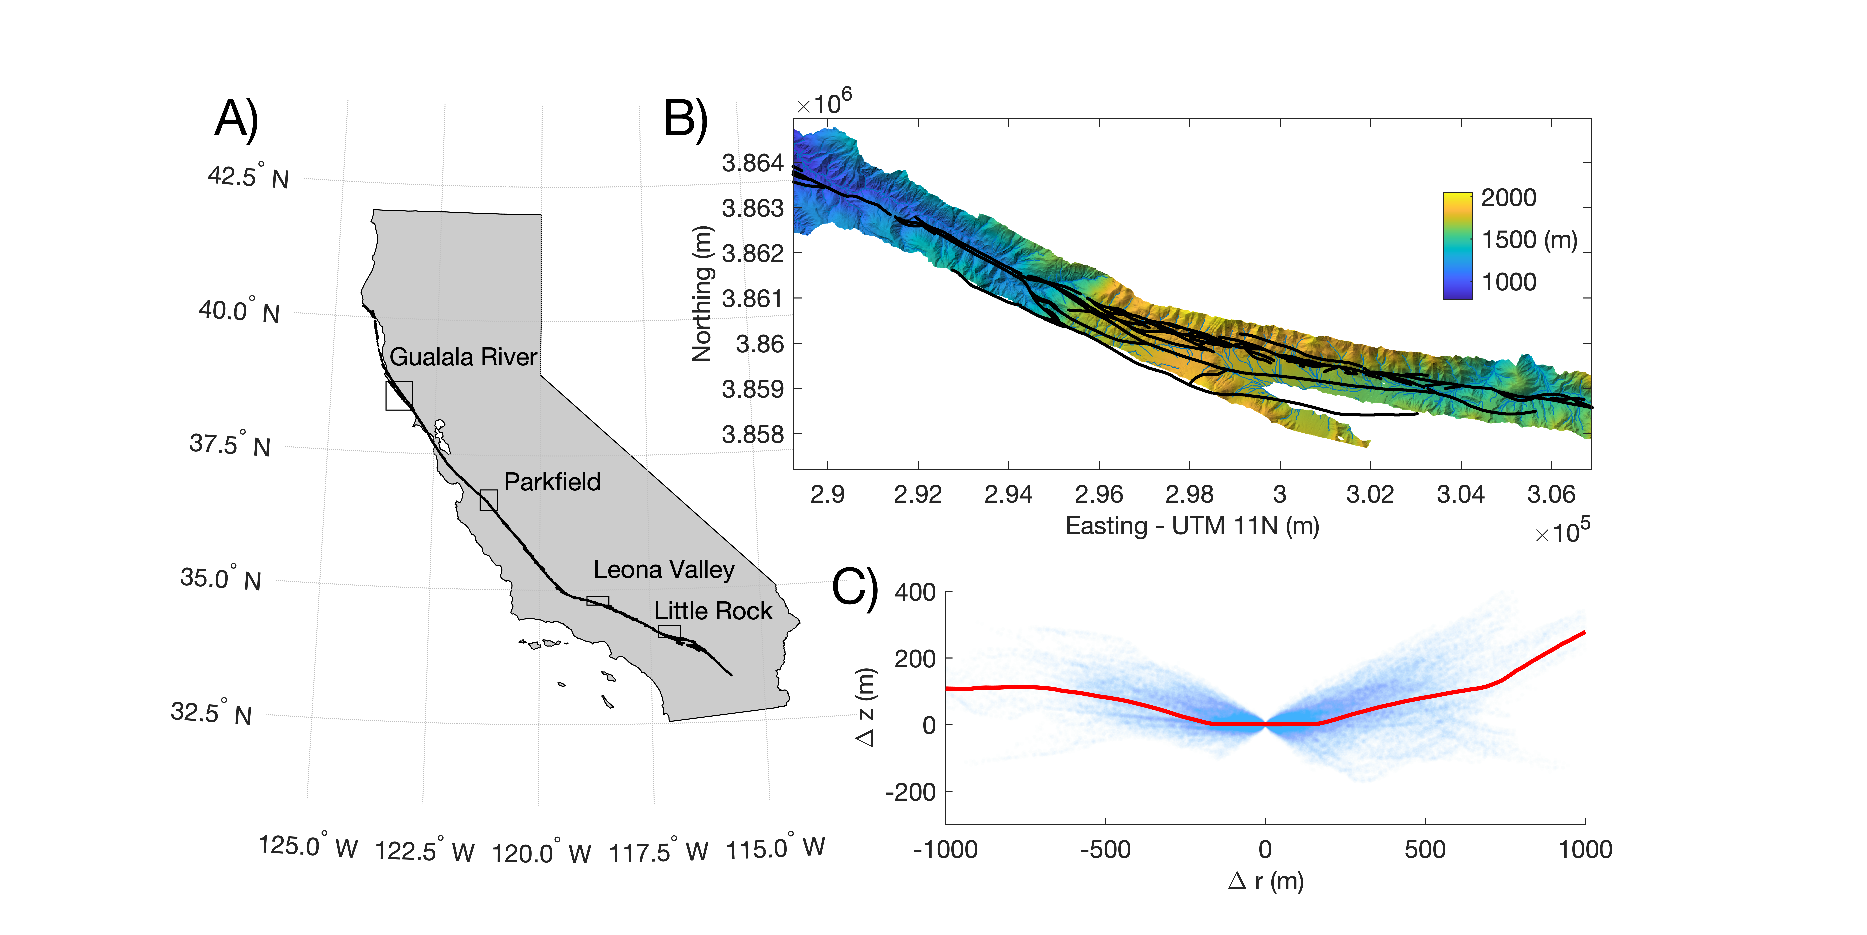
\includegraphics[trim={2.5cm 0.2cm 3.2cm 1.2cm}, clip, width = 1\textwidth ]{figures/locale_topo_combinend.eps}
    \caption{A) Map trace of the San Andreas fault. Localities featured in this proposal are identified. B) DEM derived from the B4 LIDAR project for the Leona Valley. Faults traces are overlain in black. C)  Stack of relative elevation ($\Delta z$) as a function of distance to the fault ($\Delta r$) taken from West to East. Red line indicates the median of 10m moving window through the data. Note the kinks in at $\pm100$ on either side of the fault.}
    \label{fig:overview_topo_combined}
\end{figure}

\section{Target metrics of fault damage}
% What is the general approach used to select the target metrics? 
Based on anecdotal evidence and known geomorphic tools, I have determined a preliminary list of metrics that I hypothesize to be sensitive to the presence of a fault and its damage. Target metrics will include stacked topography, normalized steepness index, and stream orientation. I will expand upon these metrics as I iterate between modeling results and ground-truth campaigns. As a proof of concept, I assessed these target metrics along the San Andreas Fault in the Leona Valley. The locale hosts a variety of fault geometries (see Figure \ref{fig:overview_topo_combined}). The mapped trace of the fault has sections that are distinctly linear, whereas others exhibit complex geometries with multiple, sub-parallel strands. Theoretical arguments and outcrop studies \cite{Faulkner2008OnFaults} suggest that this variability should correspond to diversity in the width, intensity, and character of the damage zone. 

\subsection{Stacked topography} 

Perhaps the most conspicuous features of the San Andreas are long linear valleys with rivers centered, or slightly offset from mapped fault traces. Landscape models suggest that rivers reorient along zones of weakness \cite{Roy2016}. The lateral erodability of bedrock channels running along a zone of weakness is sensitive to the strength of the bedrock \cite{Johnson2015AChannels}. The width of fault parallel valleys may be closely tied to the extent of the damage zone.

I assess this by computing the Euclidean distance and relative height difference to the nearest mapped fault trace for every point in the DEM (Figure  \ref{fig:overview_topo_combined}C). The median profile illustrates that the San Andreas is in a valley and, interestingly, exhibits kinks on either side of the fault at roughly 100m. This scale is compatible with known width estimates of the damage zone on the San Andreas fault \cite{DorGeologicalDirection}.

\subsection{Normalized steepness index} 

Bedrock channels are highly dynamic features that readily respond to climatic and tectonic forcing. Incision into the bedrock river channel is well approximated to a first order by the stream power model which assumes that the rate of erosion ($E$) is proportional to the shear stress acting on the bedrock. This can further be expressed as a power law of channel drainage area ($A$) and slope ($S$), $E = kA^mS^n$, where $k$ includes information about precipitation, the timing, and intensity of floods, and, notable to my analysis, the erosivity of the bedrock \cite{Whipple1999DynamicsNeeds}. Exponents $m$ and $n$ are empirically determined exponents. When uplift is balanced by river erosion (the steady state assumption), the normalized steepness index, $K_{sn} \equiv  [U/k]^{1/n} = A^{m/n}S$ is a tool to assess tectonic and climatic features directly from the topography. This approach has been widely used to observe large-scale patterns in regional uplift \cite{Whipple1999DynamicsNeeds, Whipple2004b}. However, a decreased normalized steepness index may also indicate a decreased erosive strength of the bedrock. Though care must be taken to not disregard uplift and precipitation patterns, I hypothesize that the normalized bedrock steepness index will record the profound changes in the strength of the bedrock induced by fault damage.

%
\begin{figure}
    \centering
    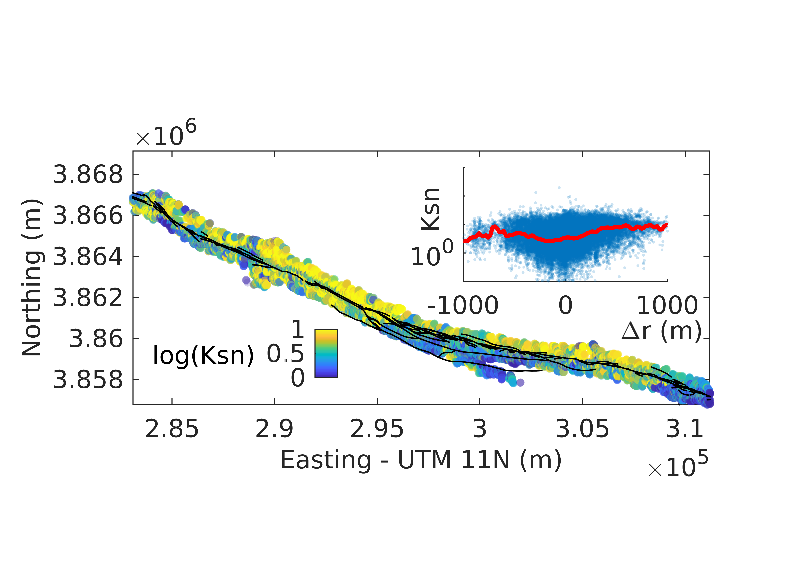
\includegraphics[trim={0.1cm 1.3cm 1.2cm 1.8cm},clip]{figures/ksn_map.eps}
    \caption{Map of the normalized steepness index for the Leona Valley. Inset shows the normalized steepness index plotted as a function of distance to the fault, $\Delta r$ (from west to east). Red line indicates a median a moving window through the data.}
    \label{fig:ksn}
\end{figure}
%

Following the stacking method employed for the previous metric, I find that a similar 100-200 m fault-perpendicular length-scale is present in the $K_{sn}$ metric (inset of Figure \ref{fig:ksn}). Remarkably, spatial patterns in low $K_{sn}$ values coincide with areas where the fault trace is more complex. 

\subsection{Stream orientation} 

River deflection and sheared basins have long been documented as an indicator of offset on an active fault. Landscape evolution models show that distributed deformation may deflect individual rivers or even entire catchments \cite{Gray2018Off-faultDrainages}. More pronounced river deflection occurs as a direct result of fault offset and the buttressing effect of shutter ridges, which, provided enough time, can lead to channel abandonment or capture \cite{DuvallDynamicEnvironment, Zielke2015FaultData}. I also expect that damage and reduced bedrock cohesion will tend to reorient rivers \cite{Roy2016}. I will test 1) whether these features are emergent and robust in a large-scale analysis and 2) how and at what scale rivers are deflected. It will be interesting to interpret these metrics in the context of distributed deformation, active faulting and fault damage. I quantify river orientation by examining the vector product of river segments to the nearest fault segment. Stacked according to distance from the fault, my observations in the Leona Valley support a pronounced deflection of the median river path towards the fault (Figure \ref{fig:river_deflection}).
%
\begin{figure}
    \centering
    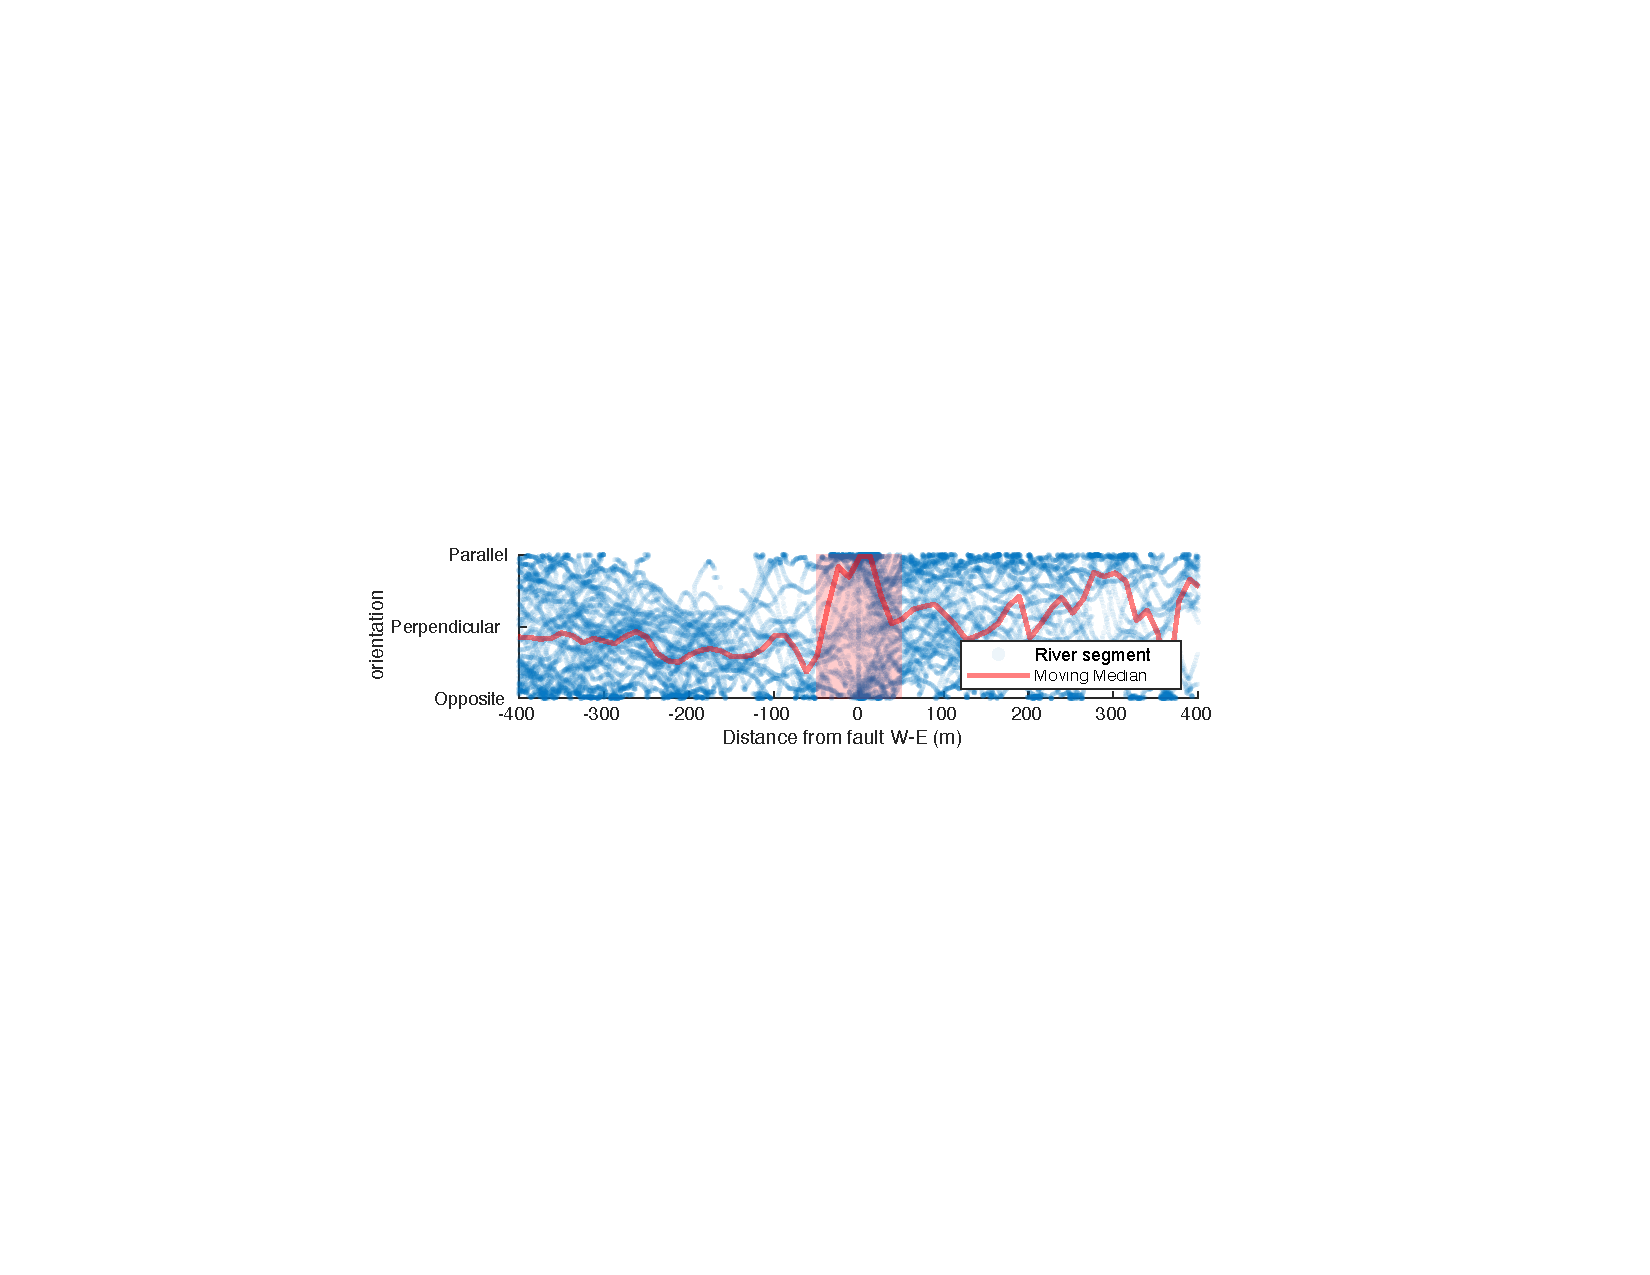
\includegraphics[scale=1]{figures/river_defelction.pdf}
    \caption{River segment orientation as a function of distance from a fault. The red line indicated the median of a 10m moving window though the data. Note the strong deflection of the river profiles around 50m on either side of the fault.}
    \label{fig:river_deflection}
\end{figure}
%
\section{Landscape evolution in the presence of a fault}
%Why use landscape evolution models?
Decoupling fault kinematics from the fault damage is the major challenge of the proposed research. Channel offset, sediment transport, and deposition, and lithological contrast make the interaction between faults and landscapes intricate; landscape evolution models provide a footing to address these interactions. Target metrics will educate modeling decisions, which in turn can lead us to emergent insight and novel ways to interrogate the landscape.

%What type of landscape evolution models exist?
Recent modeling studies set the stage for the study of faults in the landscape \cite{DuvallDynamicEnvironment, Roy2016, Gray2018Off-faultDrainages, Harbert2018TheLandscape}. \textcite{DuvallDynamicEnvironment} modeled strike-slip faults to study channel abandonment and catchment, \textcite{Roy2016} studied the role variable lithologies  (as an analog to fault damage zones) in exerting first-order controls on the orientation and characteristics of river networks, though did not include active faults in their models. \textcite{Gray2018Off-faultDrainages} reproduced deflected streams and entire catchments by modeling a zone of distributed deformation. Landscape evolution models have been implemented to understand river meandering, cratering on Mars, and mine-spoil degradation. Though the applications are remarkably diverse, landscape evolution models typically share some basic components.
 
% How does the landscape evolution model work?
Landscape evolution is well described to first order by competition between tectonic uplift and erosive agents:
%possibly a spot to save space
\begin{equation}\label{eq:evol}
    \dfrac{\partial{h}}{\partial{t}} = U - E_f - E_h
\end{equation}
where $\dfrac{\partial{h}}{\partial{t}}$ is the change of elevation with time, $U$ is the regional uplift rate. The river incision rate, $E_f$, is determined by the stream power formulation. The erosion (or deposition) rate, $E_h$, is approximated to be proportional to the slope gradient through a diffusion coefficient, ($D$), such that $E_h \sim D\nabla \boldsymbol{r}.$

 % How will I model the presence of a fault? 
I will represent a fault by assembling the existing components that represent faults, that is fault offset, fault damage, and distributed deformation. To do so, I introduce an advective term to Equation \ref{eq:evol} and make the parameterization of the erosive terms spatially variable. 

\textit{LandLab} is a rapidly growing and thoroughly tested python library providing the basic building blocks for a landscape evolution model which has just recently been developed \cite{Hobley2017}. Using \textit{LandLab} as a foundation, I reproduced the key features of a fault. Should it be necessary, \textit{LandLab} is well suited for increased sophistication (e.g., non-linear hillslope diffusion, sediment transport, etc.). Figure \ref{fig:model_out} demonstrates some preliminary models simulating both an actively slipping fault and a damage zone.

\begin{figure}
    \centering
    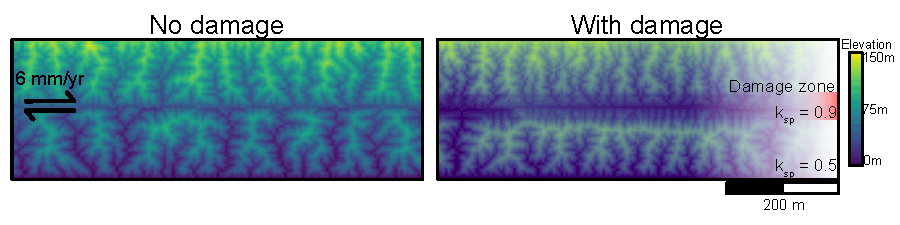
\includegraphics[scale = 1]{figures/damagezone_landscapevolution.pdf}
    \caption{Demonstration of two model end-members. A band with increased stream power $k_{sp}$ represents the damage zone. Note that the presence of the damage zone causes the shutter ridges to link and form a fault parallel valley.}
    \label{fig:model_out}
\end{figure}
 
\section{Ground-truth}

The first ground-truthing site will be Parkfield, CA on the central San Andreas where previous intensive instrumentation and study have resulted in multiple metrics of the damage zone. Trapped seismic waves, gravity measurements and magnetotellurics constrain the geometry of the damage zone at depth \cite{Thurber2003,Thurber2004Fine-scaleEarthquakes, Li1994Seismic1992}. A 3 km drill hole which directly intercepts the fault at depth and has recovered in situ samples \cite{Schleicher2006OriginCalifornia, Schleicher2009OnCalifornia}. The experiment is an unparalleled opportunity to couple surface information to measurements at depth.

I will consider two more exploratory sites that allow for direct field measurements customized to this study. The Gualala river runs in a remarkably straight line along the San Andreas fault for over 10km. Bedrock channels incising into the damage zone and draining into the Gualala may provide sites to calibrate model parameters. Little Rock, a well-studied locale for pulverized rock, and a characteristic signature of dynamic fault damage may provide an alternative field site. \textcite{Rempe2013DamageFault} conducted a detailed structural, microstructural and geophysical analysis whereby the extent and intensity of the damage zone is well characterized.

% This might be worth including particularly considering that this is NASA
Finally, I will compare our results to maps of distributed deformation collected using InSAR, differential LIDAR and image cross-correlation. Though these measurements do not directly measure of damage, it will be insightful to understand where long term damage correlates with off-fault co-seismic deformation. 

\section{Conclusion}

Fault damage is a key under-constrained aspect of earthquake rupture that affects hazard estimation and our physical understanding of the earthquake cycle and tectonics \cite{savage2011collateral, Chester2009CharacterizationGeneration,lyakhovsky2014fault,Roy2016,shipton2006missing, Faulkner2006SlipZone}. A remote sensing approach using NASA funded airborne LIDAR is likely the only economical way to detect and quantify fault damage on a broad scale. The proposed work will capture a timescale of deformation that has been inaccessible to modern geodetic measurements. The pieces of the puzzle are in place: faults are expressed in the landscape; fault damage has been characterized on active and fossil faults; there is preliminary evidence to show that geomorphic metrics detect fault damage. The proposed research simply aims to link these observations in a coherent and informed way. 

\chapter{Relaxing the constraints of earthquake statistical models: a machine learning approach}\label{cpt:ML}

\section{Introduction}

State-of-the-art statistical models build upon a lineage of earthquake phenomenoly. At the core of models such as epidemic-type aftershock sequence (ETAS) models are well-known statistical laws of seismicity, the Gutenberg Richter law, the productivity law and the Omori law of aftershock decay \cite{Knopoff1982, ogata2017statistics}. ETAS (BASS \cite{Holliday2008Self-similarSequences,Holliday2008ABASS}, and other variants) aim to measure to time-varying rate of earthquakes as a function of time. ETAS states that the rate of aftershocks is the sum of the background rate of earthquakes, along with the contribution of every single earthquake that has previously occurred \cite{Ogata1988StatisticalProcesses}. Contributions from individual earthquakes follow a time-decay. The design of statistical models which build off of these models is therefore nearly physics free. It stands to reason that physical insight from these models requires researches to relax constraints on the parameterization of the statistical laws or reassess the architecture of the statistical laws altogether.

Allowing parameters to change in space and time is an approach to solving this problem. Chapter \ref{cpt:productivity} is an example where, effectively, a single parameter, the earthquake productivity, was allowed to vary for each mainshock. A classical ETAS model for a region has 5 or 6 parameters \cite{Ogata1988}. As constraints relax the parameter space grows exponentially and without smoothing becomes under-determined. Smoothing constraints are typically physics-free. Alternatively, one may choose to compare a subset of the data with another, which at its core is a subjective decision on how to smooth the data. While it may not appear to be so, earthquake statistics rapidly become limited by data availability.

In this chapter, I will investigate an alternative approach to addressing this problem. There is some basis to suggest that machine learning approaches may outperform ETAS models. In a recent study, \textcite{VanderElst2017} tested whether the similarity to previous earthquake sequences provided a better prediction of the upcoming earthquake rate than did ETAS. While the authors did not outperform ETAS, they did find that the misjudgments of ETAS were more extreme than their model. The model of \textcite{VanderElst2017} is very similar to the well known k-nearest neighbor algorithm widely used in computer science. There is a growing body of literature that explores whether different machine learning approached can be used to predict earthquakes \cite{Last2016PredictingCountries, Adeli2009, Panakkat2007, Reyes2013, Asencio-Cortes2017, Geller1997EarthquakeReview, Morales-Esteban2010PatternSeries}. A dominant focus is attributed to assessing the magnitude of the largest event \cite{Last2016PredictingCountries,Panakkat2007,Adeli2009}. To the best of my knowledge, a proper comparison to state-of-the-art ETAS predictions is missing from these analyses. Moreover, many of these models efforts use statistical parameters as inputs to their predictions. Comparing the results of a machine learning with predictions from a random Poisson background seismicity yields a false sense of confidence. 



\section{Work plan}
The proposed work plan follows five steps. 

\subsection{The data}

In a meta-analysis, \textcite{Mignan2015} found that that in the debate about the prognostic values of foreshocks, a catalog with a low magnitude of completeness was a key differentiator between null-results and positive findings. Data availability is a limiting factor in the study of earthquake physics. Global catalogs contain on the order of $10^{4-5}$ earthquakes that are above the magnitude of completeness. Regional catalogs notably the Southern California Earthquake Data Center (SCEDC), Northern California Earthquake Center (NCEDC) and the Unified Japan Meteorological Agency feature up to $10^6$ earthquakes. All have been studied extensively. However, following a monumental template matching effort (Ross et al. 2018, SCEC abstract), the number of earthquakes in the catalog for Southern California has been increased by a factor of 13 and fully relocated. 

\subsection{The null hypothesis}

The state-of-the-art in aftershock statistics is a space-time varying ETAS model. ETAS will serve as the benchmark for this study. I hypothesize ETAS enforces strongly parameterized constraints on the space-time distribution of aftershocks and accordingly could be outperformed by a machine learning approach. A marginal prediction gain of the rate of aftershocks in an upcoming time step would be a successful implementation of the machine learning algorithm.

\subsection{The training, validation and test data}

A major pitfall of machine learning approaches is the selection of training, validating and test data. The training data is used to train our model; the validation data is used to tune hyper-parameters. The test data is used to assess the performance of the model (i.e., how good is our model?). The design of our input data is, therefore, a key feature of this study. As an overview, the input to the model will be earthquake time series and the output will be the upcoming rate of earthquakes. In order to not over-sample the background rate of seismicity, I will sub-sample the earthquake catalog to ensure an equal representation of periods where no earthquakes occur and earthquake sequences. Next, the catalog would be spatially discretized and stored into a vector containing the cumulative magnitude of the earthquakes at each discrete time step. More sophisticated approaches will be discussed below. A third of the catalog will be reserved for the validation step.

\subsection{The algorithm}

The processing outlined above turns the problem into something analogous to image processing (in this case a 1 by N `image'). Convolutional Neural Network (CNN) approaches are now widely used and considered the go-to approach for image processing. CNN's consist of a fully connected neural net preceded by a set of convolutions, decimations (or pooling) and activations which condense the input image into features learned to be significant by the network. All parameters of the CNN (weights, biases, including those in convolutional filters) are determined by stochastic gradient descent and backpropagation through the neural network. The parameter space of neural networks is very large, depending on the depth of the neural network, the number of parameters can reach many thousands. Very large data sets crucial to this approach. Various methods, cross-validation, drop-outs, and an assessment of the learning rate help prevent over-fitting the data.

\subsection{Validation}
In order to validate our model, we will generate a prediction of the rate of seismicity on the remaining third of the data. This prediction will be compared to an ETAS model calibrated in the same region.

\section{Machine learning as a tool to highlight abnormal source physics}
It will first be interesting to assess whether a Neural Network can reproduce the first order behavior of an ETAS model. Should we succeed at this first milestone, I am particularly interested in any second-order features that may arise from this analysis. Specifically, I expect to gain particular insight into the physics of earthquake occurrence at places or periods where the performance of a CNN is increased relative to an ETAS. This approach highlights periods in time (or places) where the failures of ETAS are not simply the result of the randomness and stochasticity of the system. This research approach contends that the failure of ETAS models likely correlates with earthquake predictability. This same reasoning led to short term predictability along the East Pacific Rise transform \cite{McGuireForeshockFaults}. 

\chapter{Project Schedule and Milestones}\label{cpt:plan}

The proposed work will be completed over 3 years (completed by 07/31/2022). The detailed schedule for the proposed research and anticipated milestones are:

\section*{2019-2020}
\textit{Wrap up aftershocks productivity project.} Submit a letter-format manuscript summarizing Chapter \ref{cpt:productivity} by the end of the spring quarter (2019).

\textit{Validation.} Validate target metrics by comparing the measurements to model results and the geophysical data available from Parkfield. Refine numerical model to include distributed deformation and sediment transport.

\textit{Null hypothesis for Californian seismicity.} Apply a non-stationary ETAS model for Southern Californian seismicity (likely incorporating existing work)

\textit{}

\subsection*{Specific questions to be answered:}
\begin{enumerate}
    \item What landscapes metrics are sensitive to fault damage?
    \item Do geophysical estimates of damage zone width (Parkfield) correspond to those extracted from the landscapes?
    \item How well do current statistical laws characterize the seismicity of Southern California?
\end{enumerate}

Milestones: Qualification exam, second-year talk, submit earthquake productivity manuscript.

\section*{2020-2021}

\textit{Calibration of geomorphic metrics.} I will explore the potential of the Gualala River and Little Rock field sites to calibrate and generally educate my target metrics and model parameters. Write a paper about the case studies of either (or both) case studies of the Gualala River and Little Rock field sites

\textit{Convolutional neural network.} Design and test the architecture of the neural network that will be used to evaluate the seismicity rate. This will involve acquiring data, designing the input data structure, and determine the best model framework for the task.


\subsection*{Specific questions to be answered:}
\begin{enumerate}
    \item How does co-seismic deformation correspond to long-term damage?
    \item What is the quantitative mapping between remotely sensed metric and physical features of the crust (e.g., cohesion, elastic moduli)?
    \item What is the rate of seismicity predicted by a convolutional neural network.
\end{enumerate}

Milestone: Finish courses

\section*{2021-2022}

\textit{Upscale and Synthesis of the damage zone geomorphology work.} Upscale geomorphic detection to entire San Andreas Fault network and other NASA LIDAR products covering active faults. Write a paper on the synthesis of large-scale results.

\textit{Interpretation and synthesis of Chapter 3}

\subsection*{Specific questions to be answered:}
\begin{enumerate}
    \item How do damage zones subsume earthquake energy?
    \item How do damage zones distribute deformation in the crust?
    \item The impact on earthquake hazard: how do damage zones reflect/affect the long term hazard of the Earth’s Crustal system
    \item What are the physical implications of the relative performance of the ETAS and a machine learning approach.
\end{enumerate}

Milestone: Submit thesis and defend 

{\footnotesize
\printbibliography}

\end{document}
